
\chapter{Steady State Sinusoidal Analysis}


\section{Sinusoids}

A sinusoid is a time function of the form
\[
  A \sin(\omega t + \phi)
\]
where


\vspace{0.2in}
\begin{tabular}{c|l|l}
Name    & Meaning  & Units\\\hline
$A$   &  Amplitude  &  Volts, Amps, etc \\
$\omega$   & Frequency  & $rad/sec$ \\
$t$     & Time  & $sec$  \\
$\phi$  & Phase & $rad$  \\
\end{tabular}

\vspace{0.2in}
Sinusoids arise in ECE through two primary ways
\begin{enumerate}

\item The mathematical solutions to circuits built-up of R, L, C elements sometimes
contain sinusoidal terms.

\item Rotating machines like generators primarily generate sinusoidal voltages.   Our regular wall outlets
have a sinusoidal voltage with frequency 60 Hertz, 377 rad/sec.

\end{enumerate}


Some properties of sinusoids include:

\begin{itemize}

\item Since $\omega$ is in $rad/sec$, we must frequently convert frequencies in cycles per second (Hertz)
by noting that one cycle is $2\pi$ radians. Thus for example:

  \[
    1000 Hz = 2\pi\times 1000 \approx 6283.2 rad/sec
    \]

\item The Phase angle, $\phi$, slides the sinusoid back and forth along the time axis acording to its value
(which is a constant).  There are special cases when $\phi$ is a multiple of $\pi/2$ such as
\[
  A \sin(\omega t + \pi/2) = -A \cos(\omega t)
  \]

or
\[
  A \sin(\omega t + \pi) = -A \sin(\omega t)
  \]
according to various trig identities.

\item Since $\sin()$ and $\cos()$ have important geometrical interpretations, it is not surprising that it is often useful to
visualize a sinusoid as a projection of a rotating vector onto the $X$ or $Y$ axis.

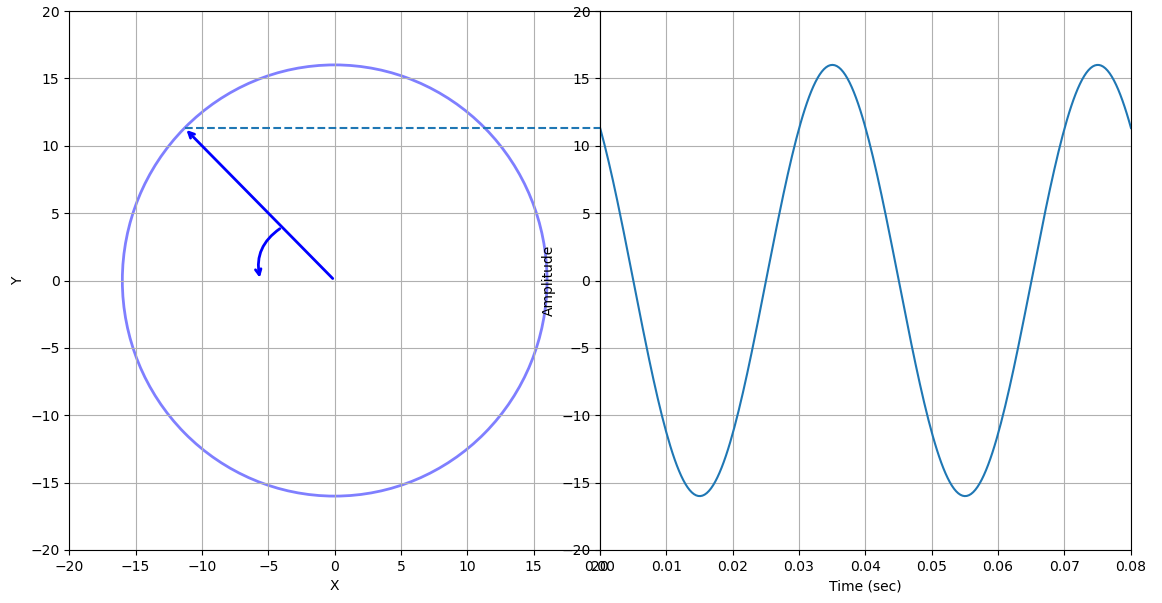
\includegraphics[width=0.5\textwidth]{figsChapt02/MQ41BN01.png}

In the left panel, a vector rotates counter-clockwise at rate $\omega$ radians
per second.   If we trace the y component of the vector over time, we get the
sinusoid appearing on the right.
\href {https://youtu.be/a_zReGTxdlQ?si=hQbJcQvjlW3IVkuE&t=73} {[Animation from Kahn Academy]}

\end{itemize}

\subsection*{Sinusoid Review Problems}

\subsubsection*{basic functions}
For the following graph,

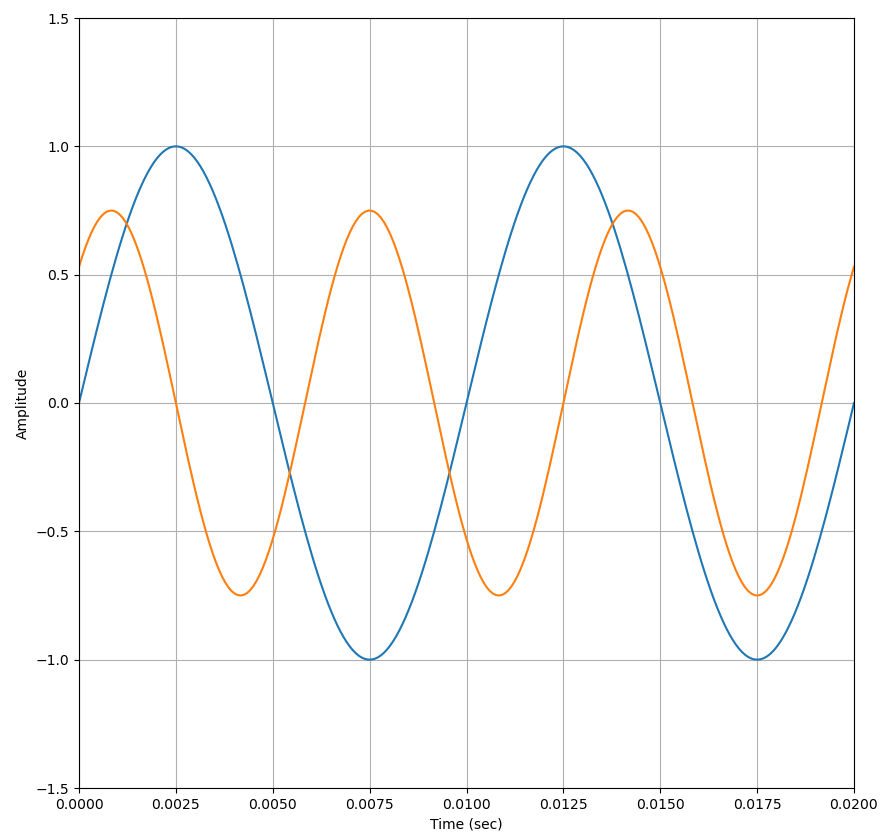
\includegraphics[width=0.5\textwidth]{figsChapt02/MQ41BN02.png}

\paragraph{Problem:}
Find the equation of the two sinusoids.

\paragraph{Solution:}

Looking at corresponding peaks or zero-crossings of the blue trace, the amplitude, $A$, is 1.0, and
the period, $P$,   is 0.01 seconds so using:

\[
P  =  2\pi/\omega_{bl}
\]
\[
  \omega_{bl} = 2\pi/0.01 = 628.3 \;rad/sec
\]

at $t=0, \sin(\omega_{bl}t + \phi_{bl}) = 0$ so $\phi_{bl} = 0$, and the equation is:
  \[
    y_b(t) = 1.0\sin(628.3t)
    \]
For the orange wave, the amplitude is 0.75 and checking the time of the 3rd and 2nd peaks
(or any 2 successive peaks):
\[
P = 0.0142 - 0.0075 = 0.0067 sec
\]

\[
  \omega_o = 2\pi/0.0067 = 937.8 \;rad/sec
\]
reading the graph,
at $t=0$, $\sin(\omega_ot + \phi_o) = 0.5$ so at $t=0$, $\sin(\phi_o) = 0.5/0.75 \; \to \; \phi_o = 0.73 rad \approx 42^\circ$,
so the equation is
\[
y_o(t) = 0.75\sin(937.8t+ 0.73)
\]



{\bf Additional Problems:}

\begin{enumerate}


\item  {\bf Problem:}
For both the orange and blue waves, find time where $\theta = \omega t+\phi =  0$ (using $\sin(0) = 0$):

{\bf Solution:}\\
    Blue: $\omega_{bl} t + \phi_{bl} = 0$ plugging in values above, we have $628.3t+0=0 \; \to\; t = 0$.\\
    Orange: $\omega_o t + \phi_o = 0$ plugging in values above, we have $937.8t+0.730=0, t = \frac{-0.730}{937.8}=-.00078$,  this value is not plotted but adding one half period gives $t=-0.00078+0.0067/2 =0.00257$


\item {\bf Problem:} Also for both waves, find time where $\theta = \pi/2$ (using $\sin(\pi/2)=1$)

  {\bf Solution:}\\
    Blue: $628.3t+0=\pi/2\;\to\;t = 0.0025$\\
    Orange: $937.8t+0.73 = \pi/2\;\to\;t=0.000897$

\item Check the above solutions by inspection of the graphs.
\end{enumerate}




\subsection{Phase Shifts }  Looking back at the blue and orange waves, We can see that there is a
phase difference between them, and we derived that it was 0.73 radians.
Recalling the equations of our two waves:
\[
y_b(t) = 1.0\sin(628.3t)
\]
\[
y_o(t) = 0.75\sin(937.8t+ 0.73)
\]
Let's consider $y_b(t)$ the ``reference'' wave.

Note that in comparing any two waves, we can set the
phase shift of one of them to zero (unless there is some additional time reference).  For example
if

\[
y_1(t) = 1.0\sin(200t - \pi)
\]
\[
y_2(t) = 0.75\sin(200t +\pi/2)
\]
The following two sinusoids have the same relationship to each other:
\[
y_1(t) = 1.0\sin(200t + 0)
\]
\[
y_2(t) = 0.75\sin(200t + 3\pi/2)
\]
(we have added $\pi$ to both arguments.)

\paragraph{Phase Lag and Phase Lead}

Definition:

\begin{quotation}
If the phase shift of wave B with respect to wave A is $\phi>0$, then
wave B {\bf leads} wave A.
\end{quotation}


Definition:

\begin{quotation}
If the phase shift of wave B with respect to wave A is $\phi<0$, then
wave B {\bf lags} wave A.
\end{quotation}


Referring back to the blue and orange waves above, the phase shift of the orange
wave compared to the blue wave is positive ($+0.73rad$) so the orange wave {\bf leads} the
blue wave.  Indeed it  peaks earlier in time than the blue wave does.



\subsection{Sum of 2 sinusoids}
\paragraph{Example:}

{\bf Problem: }
\[
V(t) = 8\cos(\omega t + \pi/3) + 4\cos(\omega t)
\]

{\bf Solution: }

Note that each sinusoid can be considered to be a projection of a rotating vector:


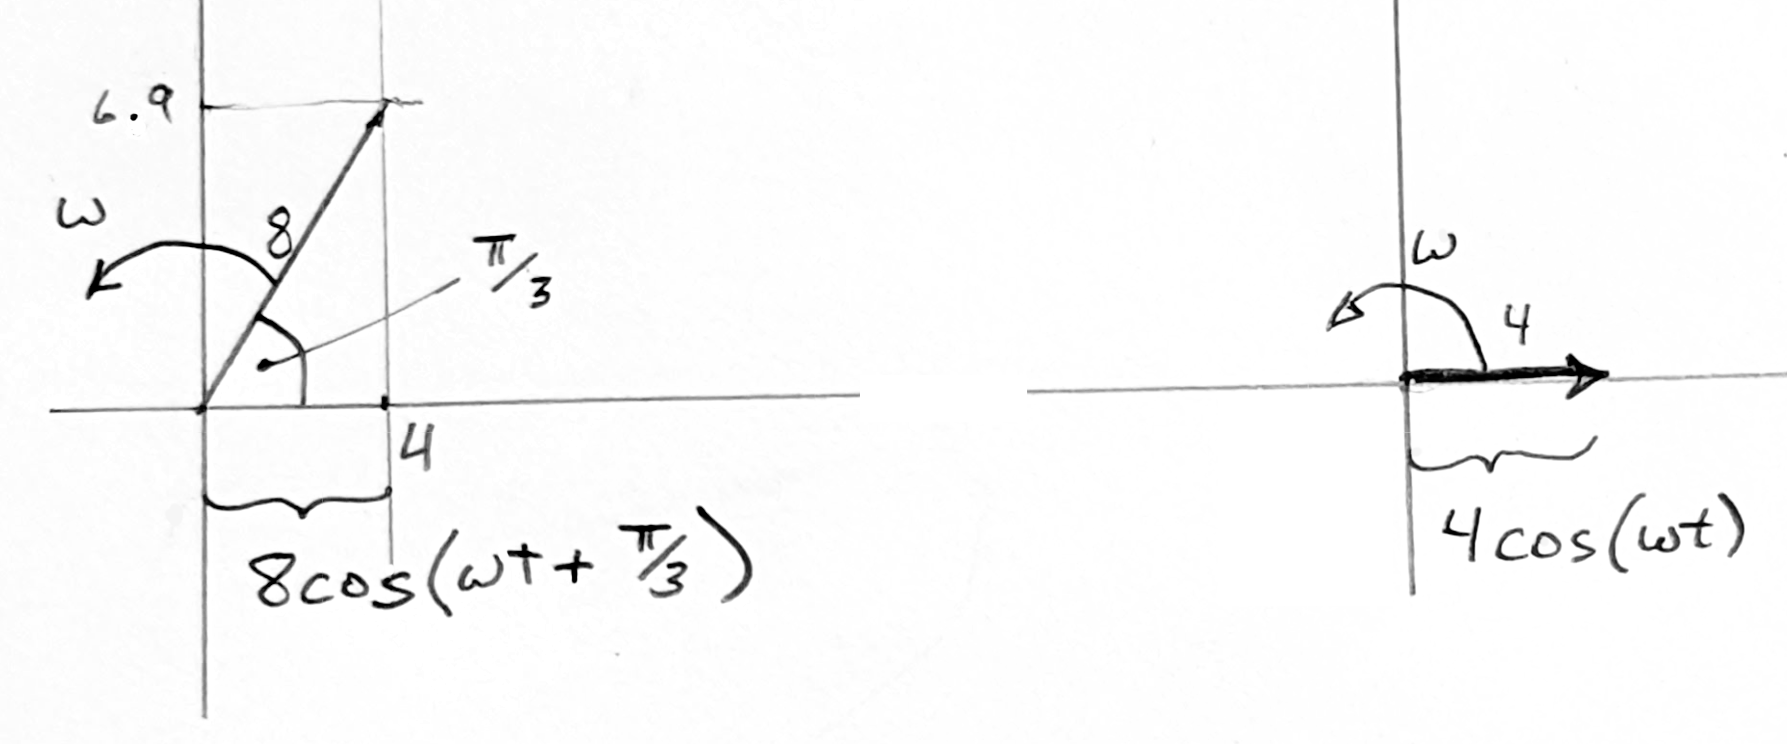
\includegraphics[width=\textwidth]{figsChapt02/KG21706.png}

Therefore, their sum is the projection of their vector sum:

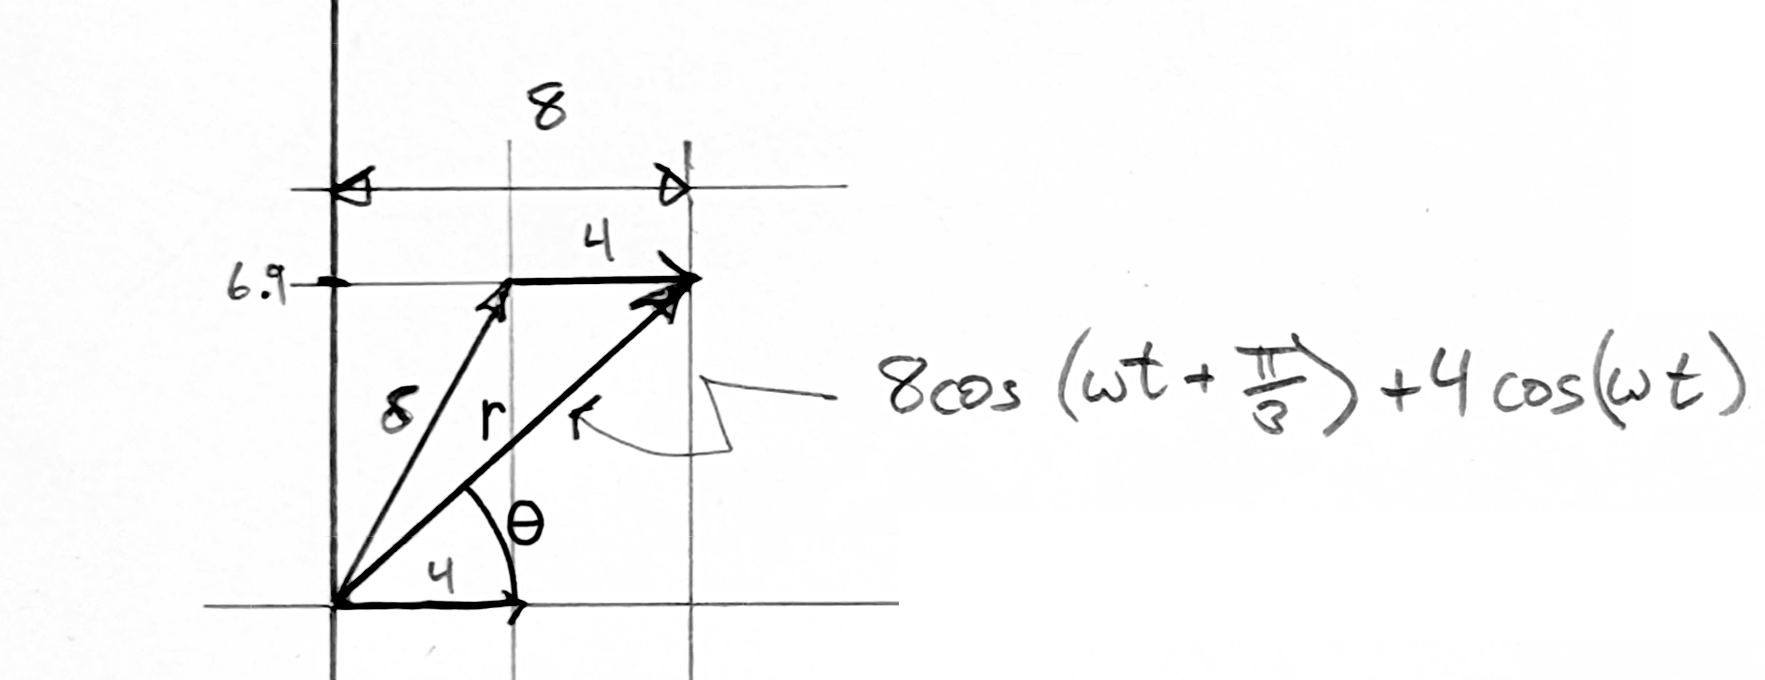
\includegraphics[width=.8\textwidth]{figsChapt02/NE94010.png}

\[
r = \sqrt{(8\sin(\pi/3))^2+8^2} = 10.56,\quad \theta = \mathrm{atan2}(6.9, 8) = 40.8^\circ
\]



\section{LODE Analysis of Electric Circuits  }


First we start with the
``Conventional Method'' (from the 1800's and early 1900's).   This will involve writing
a linear ordinary differential equation (``LODE'') for the circuit, and solving using
older techniques such as assuming the form of a solution and solving for constants.
Such solutions are often divided into two components which are added to get the solution:  the ``Forced Response''
and the ``Natural Response''.

The Forced Response is mathematically of the same form as the input to the circuit. For example,
if a DC voltage is supplied to the circuit via a switch thrown at $t=0$, the forced response
has the form of a   step function.

The Natural Response has the form that depends on the system properties.  For example,
a system which resonates in response to a transient input may have a transient response consisting
of a sinusoid which is multiplied by a damping function so that it disappears (declines in amplitude)
over time such as
\[
v_{NR}(t) =e^{-.1t} [ 10 \sin(45t+\pi/6) ]
\]
By about $t=100$, the $e^{-.1t}$ term is negligible and $v_{NR}(t)\approx 0$.


\paragraph{Steady State Case:}
Sometimes we care mostly about the transient ``Natural Response'', but other times (like this chapter) we care primarily
about the  ``Forced Response''.   A big application of sinusoidal steady state analysis is power
systems.  Although transients in power are also important, many loads are running far longer than
their transient time constants --- much more energy is consumed in the steady state when you turn
on a light bulb and run it for 12 hours.



\subsection{An Electrical AC Circuit}

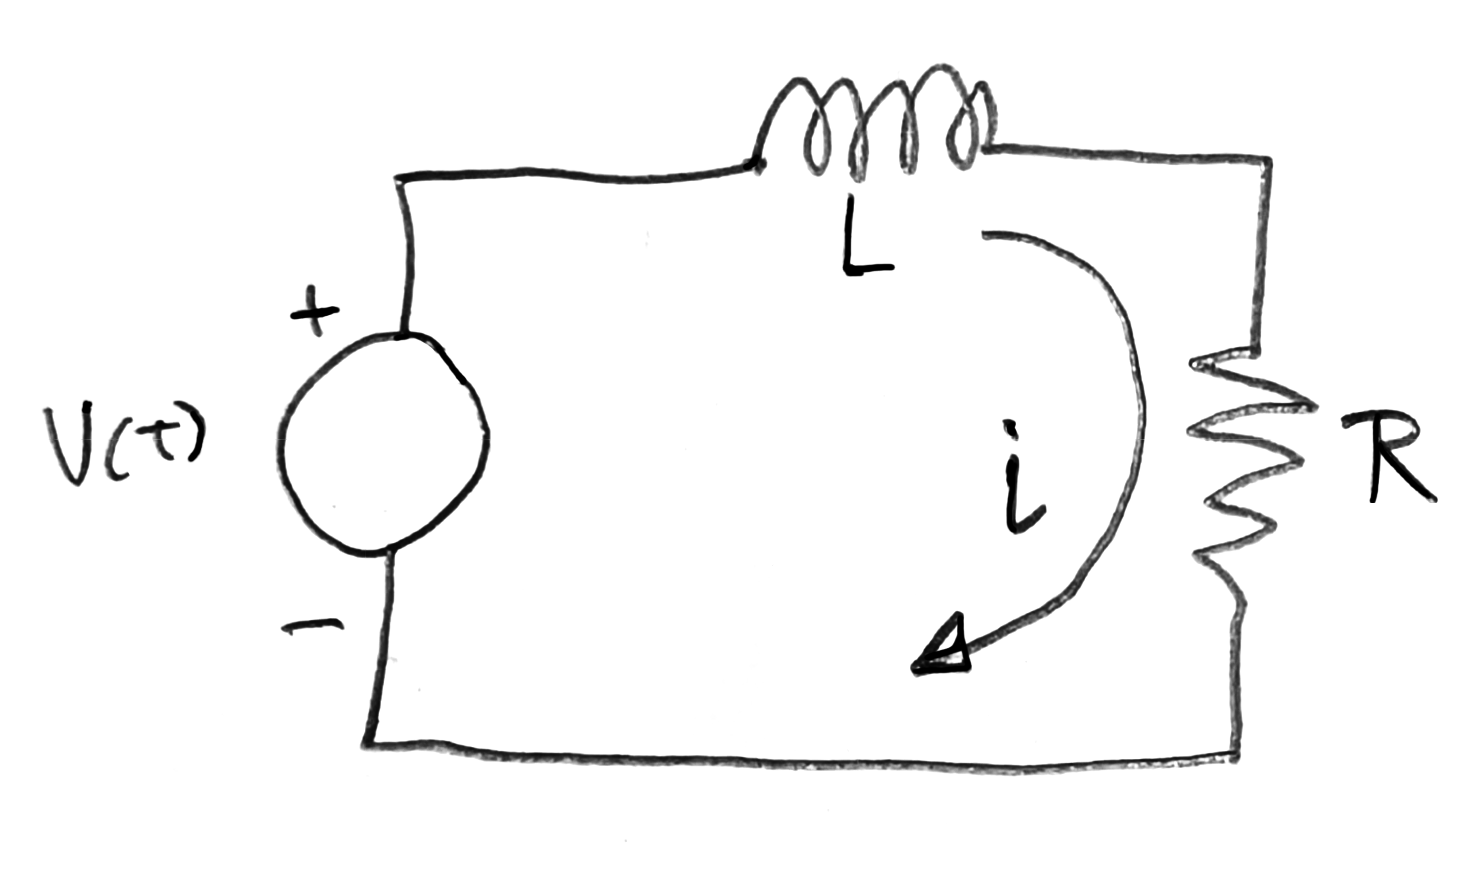
\includegraphics[width=0.5\textwidth]{figsChapt02/DI63347.png}


The traditional method for solving the response of a LODE system to sinusoidal input is roughly
introduced.

\noindent
First we take a high level look at the method:

\begin{enumerate}
\item Our Differential equation is:
\[
V(t) = L\frac{di}{dt} + iR
\]
(which is a L.O.D.E)

\item {\it assume} $\hat{i} = A\cos\omega t + B\sin\omega t$

\begin{quotation}
Q: Why is that a good assumption?

A: Because $\frac{d}{dt}\sin(x) = \cos(x)$, $\frac{d}{dt}\cos(x) = -\sin(x)$

Q: What about ``natural response''?

A: Were ignoring it!

Q: Why can we ignore natural response?

A: Because here we are studying only ``steady state response'' ... by definition this is
the same functional form as the forced response.
\end{quotation}

\item Plug   $\hat{i}$ into the LODE.

\item Evaluate derivative(s) in the LODE, collect $\sin$, $\cos$ terms

\item Solve for $A$, $B$ in terms of constants or variables in the LODE such as $R$, $L$, $V_M$, $\phi$

\item Massage the result into form $\underline{I}\cos(\omega t + \phi)$
if desired.
\end{enumerate}

\vspace{0.25in}

\noindent
Now the details:

\begin{enumerate}
\item Our LODE is:
\[
V_M\cos\omega t = L\frac{di}{dt} + iR
\]

\item We assume the solution is:
\[
\hat{i} = A\cos\omega t + B\sin\omega t
\]

\[\frac{d\hat{i} } {dt} = -A\omega\sin\omega t + B\omega\cos\omega t
\]

\item
\[
V_M\cos\omega t = -A\omega L\sin\omega t + B\omega L\cos\omega t + AR\cos\omega t + BR\sin\omega t
\]

\item
\[
V_M\cos\omega t = (BR - A\omega L)\sin\omega t + (AR + B\omega L)\cos\omega t
\]

Collecting the terms and equating like trig functions:
\[
BR - A\omega L = 0
\]

\[
AR + B\omega L - V_M = 0
\]

\item
\[
A = \frac{RV_M} {R^2 + \omega^2L^2}
\]

\[
B = \frac{\omega LV_M}{R^2 + \omega^2L^2}
\]

\[
i = \frac{V_M}{R^2 + \omega^2L^2}[R\cos\omega t + \omega L\sin\omega t]
\]

\item Convert to 2 cosine waves with trig identity; Vector addition

\[
R\cos\omega t + \omega L\sin\omega t = R\cos\omega t + \omega L\cos(\omega t - \pi/2)
\]

\noindent Result:

$\sqrt{R^2 + \omega^2L^2}\cos(\omega t + \tan^{-1}(\omega L/R))$

$\omega L\cos(\omega t - \pi/2)$

$i = \frac{V_M}{\sqrt{R^2 + \omega^2L^2}}\cos(\omega t - \tan^{-1}(\omega L/R))$
\end{enumerate}

\noindent
{\bf Pretty painful!}




\section{Complex Sinusoids and Phasors  }

Consider the a complex time function:  $e^{j\omega t}$
Using Euler's equation\footnote{BTW, Euler's equation is very easy to prove using the Taylor series
expansions of $e^x, \cos(x), \sin(x)$},

\[
e^{j\omega t} = \cos(\omega t) + j\sin(\omega t)
\]

More generally
\[
Ae^{j(\omega t + \phi)} = A\cos(\omega t + \phi) + jA\sin(\omega t + \phi)
\]

We call this a ``complex sinusoid''.
The real part and the imaginary part are
both sinusoids and they are $\pi/2$ out of phase because $\sin(x) = \cos(x+\pi/2)$.

Recall that the real part of a complex number is plotted on the $x$ axis
of the complex plane (often called the real axis) and the imaginary part
on the $y$ axis (often called the imaginary axis).   So the complex sinusoid
is also a vector in the complex plane
of magnitude $A$ rotating counter-clockwise around the origin ($0+j0$),
and if $V$ is a complex sinusoid, $Ae^{j(\omega t+\phi)}$,
then $\text{Re}\{V\} = A\cos(\omega t + \phi)$
which is a regular sinusoid.

We will find complex sinusoids quite useful to simplify the process of solving
for AC sinusoidal steady state responses of circuits.


\subsection*{Better Method - Phasors (Steinmetz - not Star Trek!)}

Developed by Charles Steinmetz in 1893, we
define a {\it phasor}, $\vec{P}$ as
\[
    \vec{P} = P_M e^{j\phi}
\]

``Phasor'' is a contraction of ``PHASE vecTOR,''
but it also encodes amplitude, $P_M$.

Let's go back to the complex sinusoid
\[
Ae^{j(\omega t + \phi)} = A\cos(\omega t + \phi) + jA\sin(\omega t + \phi)
\]

We can factor the LHS above as
\[
e^{j(\omega t)}Ae^{j\phi} = e^{j(\omega t)}\vec{P}
\]
where $\vec{P}=P_Me^{j\phi}$ is the phasor which breaks down a complex
sinusoid into the product of a phasor and a
complex sinusoid of unit mag at zero phase.

The physical variable such as sinusoidal voltage or current is represented by
the {\bf real} part of the complex sinusoid,
 $\text{Re}\{V_M e^{j\phi} \cdot e^{j\omega t}\} = \text{Re}\{V_M e^{j(\omega t+\phi)}\}$
= $V_M\cos(\omega t + \phi)$

To clarify, we note that the {\bf phasor} is just a complex number:
\[
\vec{P} = a + jb
\]
and the {\bf complex sinusoid} is (assuming it is a voltage):
\[
\vec{V(t)} = \vec{V}e^{j\omega t} = V_Me^{j\phi}e^{j\omega t} = V_M [\cos(\omega t + \phi)+j\sin(\omega t + \phi)]
\]
The phasor encodes the magnitude and phase of the sinusoid but not its frequency. Also, the
complex sinusoid is a time function and the phasor is a complex constant.

\begin{ExampleSmall}
What Phasor corresponds to the sinusoidal physical voltage:
$V(t) = V_M\cos(\omega t + \phi)$?

\vspace{0.25in}
\paragraph{Solution:}
The corresponding complex sinusoid version is
\[
V(t) =\text{Re}\{V_M[\cos(\omega t+\phi) + j\sin(\omega t+\phi)]\} = V_M\cos(\omega t+\phi)
\]
Starting with the complex sinusoid, we use the fact that a phasor encodes the magnitude and phase
but not $\omega t$.
Writing the phasor form of our complex sinusoid:
\[
    V_M[\cos(\omega t+\phi) + j\sin(\omega t+\phi)] = V_M e^{j(\omega t+\phi)}
     = V_M e^{j\phi}e^{j\omega t}
     = \vec{V}e^{j\omega t}
\]
thus the phasor corresponding to $V(t)$ is
\[
\vec{V}=V_Me^{j\phi}
\]

\end{ExampleSmall}
\vfill

\begin{ExampleSmall}
What phasor corresponds to:
\[
I(t) = \cos(\omega t+\pi/4) + 2\sin(\omega t)
\]


\paragraph{Solution:} The two terms can be expressed as complex sinusoids from
which we derive phasors:

\noindent{1) First, we use our knowledge of trig functions to convert the original
function to:}

\[
I(t) = \cos(\omega t+\pi/4) + 2\cos(\omega t-\pi)
\]

$\cos(\theta)$ is the function which gives the real part of complex sinusoids.

\noindent{2)}
\[
\cos(\omega t+\pi/4)= \text{Re}\{e^{j\omega t}\vec{P_1}\}
\]
where $P_1 = 1e^{j\pi/4} = 0.707 + j0.707$.


\noindent{3)}
\[
2\cos(\omega t-\pi) = \text{Re}\{e^{j\omega t}\vec{P_2}\}
\]
where $P_2 = 2e^{j(-\pi)} = -2 + j0$.

We can also put the original complex sinusoid together as
\[
    I(t) = \text{Re}\{e^{j\omega t}\vec{P_1}+e^{j\omega t}\vec{P_2}\}
    \]

Now, comes the key benefit of phasors: we can factor out the first term of each
sinusoid:

\[
I(t) = \text{Re}\{e^{j\omega t}\left (
        \vec{P_1}+\vec{P_2}
        \right ) \}
\]
\[
\vec{P_1}+\vec{P_2} = -1.293 + j0.707
\]
so the phasor corresponding to $\vec{I}$ is $ -1.293 + j0.707$,
\[
|\vec{I}| = \sqrt{-1.293^2+.707^2} = 4.716
\]
\[
\angle{\vec{I}} = \mathrm{atan2}(.707, -1.293) = 151.3^\circ  =2.641
\]
So our phasor is
\[
\vec{I}(t) = 4.716e^{j2.641}
\]

We have reduced the problem of adding two sinusoids of different magnitudes and
phases (but not different frequencies) to adding two complex numbers.
\end{ExampleSmall}



\begin{ExampleSmall}\label{firstPhasorCktKVL}

Now we go back to the same RL circuit:

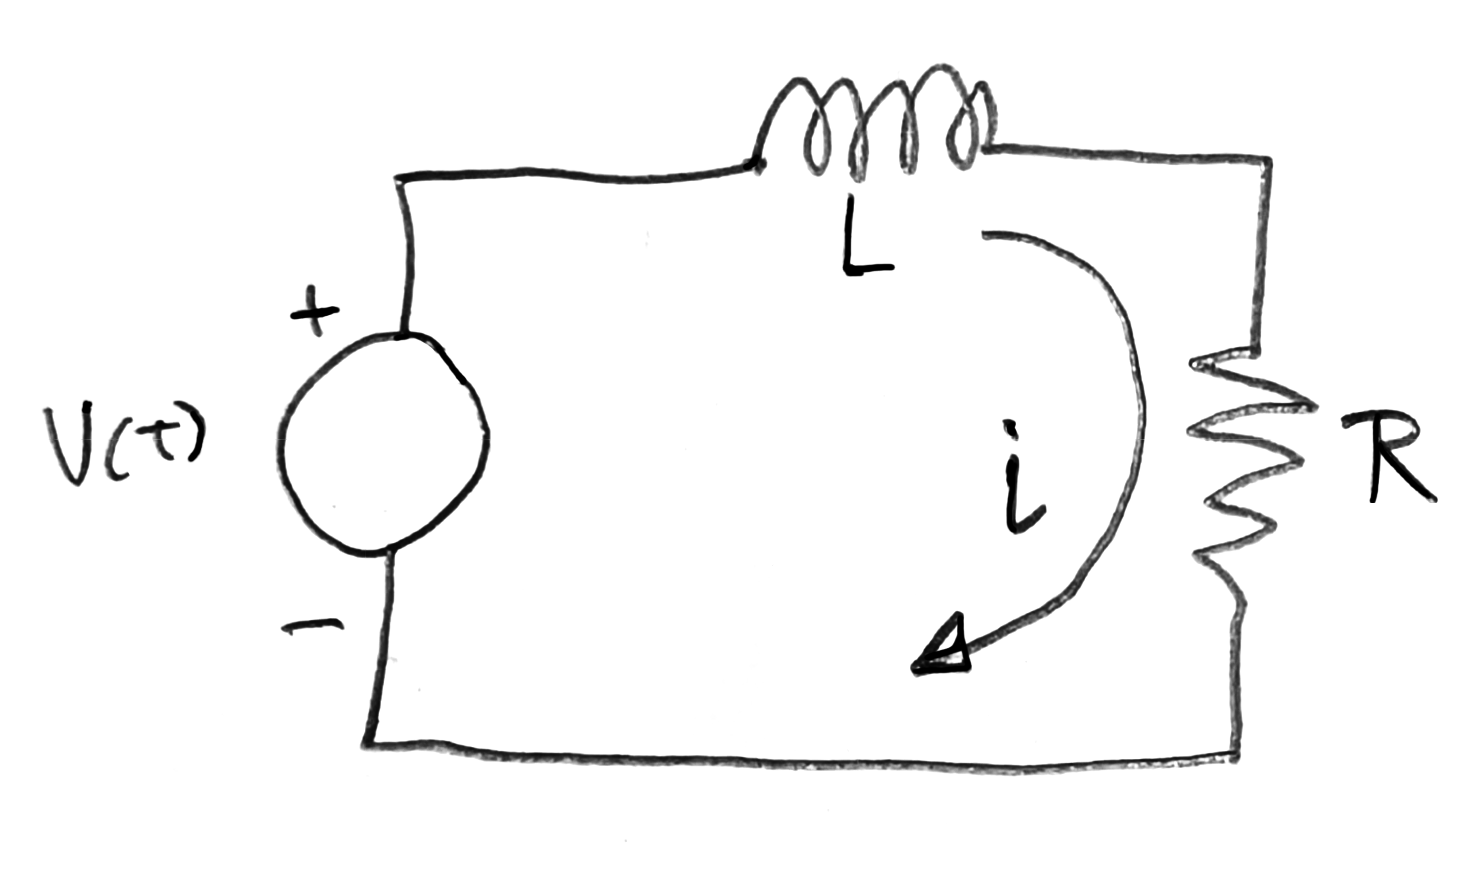
\includegraphics[width=0.5\textwidth]{figsChapt02/DI63347.png}

\begin{enumerate}
\item Summing the  voltages around the loop:

\[
V_M\cos(\omega t) - L\frac{di}{dt} - iR = 0
\]

\[
V_M\cos(\omega t) = L\frac{di}{dt} + iR
\]

\item Consider input voltage to be the real part of a complex phasor:

\[
V_M\cos(\omega t) = \mathrm{Re}\{ \vec{V}e^{j\omega t} \}
\]
And we define
\[
i(t) = \mathrm{Re}\{ \vec{I}e^{j\omega t}  \}
\]
as the current phasor which is
unknown.

% \noindent $\{i \cdot \vec{V}, \vec{I}, V_0\}$

\item We plug the unknown current and voltage phasors into (1)

\[
\vec{V}e^{j\omega t} = j\omega L\vec{I}e^{j\omega t} + R\vec{I}e^{j\omega t}
\]
(the leading $j\omega$ term on the RHS comes from differentiating as in the original LODE).


\item We can skip steps 4-6 of the previous method by
simply factoring out and cancelling $e^{j\omega t}$ from all the terms!
\[
\vec{V} = j\omega L\vec{I} + R\vec{I}
\]
(the big speedup comes when we learn to write this from
directly looking at the circuit)

We often assume zero phase angle for input sinusoids so in this (common) case we have
\[
\vec{V} =V_Me^{j0} = V_M
\]
\end{enumerate}
\end{ExampleSmall}

\begin{ExampleCont}

Solving the phasor equation we easily get:
\[
\vec{I} = \frac{\vec{V}}{  j\omega L + R}
\]

Let
\[
\phi = \tan^{-1}\left(\frac{\omega L}{R}\right)
\]
so
\[
\vec{I} = \frac{V_M}{\sqrt{R^2+\omega^2L^2}}e^{-j\phi}
\]

\[
= \frac{\vec{V}}{\sqrt{R^2+\omega^2L^2}} = \frac{V_M}{\sqrt{R^2+\omega^2L^2}}\cos(\omega t - \phi)
\]
Usually, all we really need to know is the magnitude and phase angle of our answer which we read
off directly from the phasor $\vec{I}$.
\end{ExampleCont}

Now we will directly apply the phasor method to a slightly different problem on
the same circuit:




\begin{ExampleSmall}


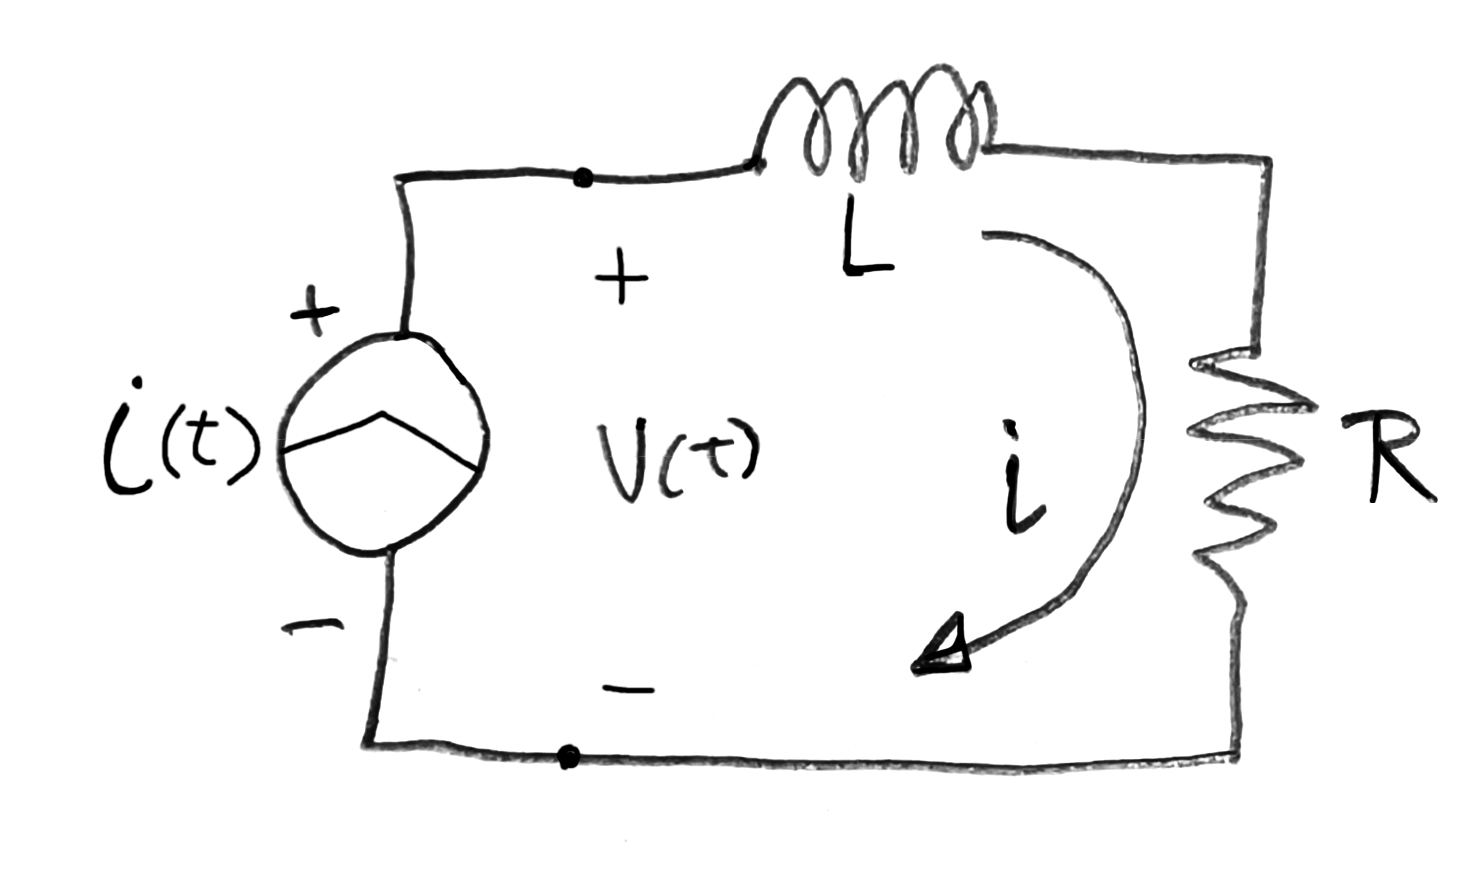
\includegraphics[width=0.5\textwidth]{figsChapt02/ND14529.png}

We drive the RL circuit this time with a current source having
\[
\vec{I} = I_me^{j0}
\]
Find the voltage $v(t)$ by the Phasor method.

\paragraph{Solution:}

Our new streamlined procedure for the steady state sinusoidal analysis is therefore
to compute each voltage drop by the product of the current phasor and the impedance,
and then write a KVL equation:
\begin{enumerate}
\item KVL Equation:

$+V_M\cos(\omega t) = L\frac{di}{dt} + \frac{1}{C}\int i\,dt + iR$

\item Convert voltage and currents to Phasor

$V_M\cos(\omega t) =$

$= \vec{V}e^{j\omega t} = \vec{I}e^{j\omega t}$

\item Plug in
\[
\vec{V}e^{j\omega t} = j\omega L\vec{I}e^{j\omega t} + \frac{1}{j\omega C}\vec{I}e^{j\omega t} + \vec{I}Re^{j\omega t}
\]


\end{enumerate}

\end{ExampleSmall}


\section{Phasor equations for energy storage components}


\subsection{Capacitor}



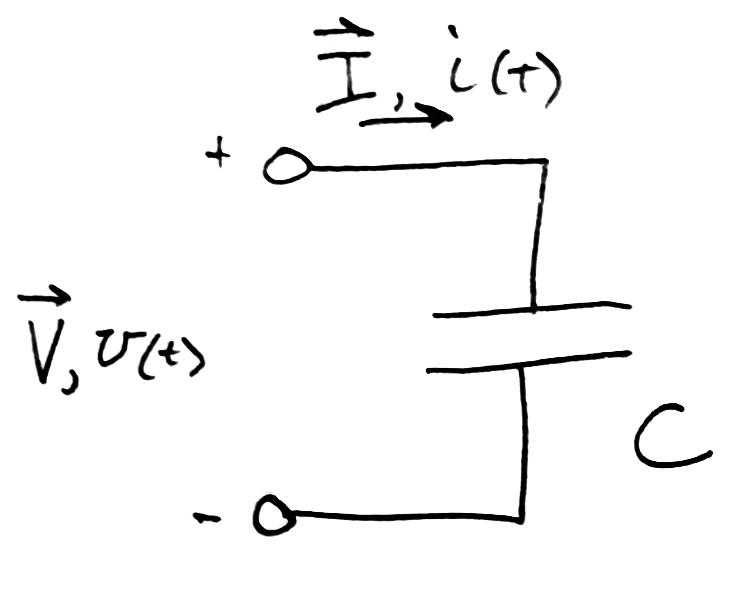
\includegraphics[width=0.35\textwidth]{figsChapt02/MI65790.png}

We know the differential equation relating voltage and current on a capacitor is
\[
v(t) = \frac {1}  {C}\int i(t) dt
\]
let's substitute a voltage complex sinusoid for the LHS, and plug in a complex sinusoid $\vec{I}e^{j\omega t}$
on the RHS:
\[
\mathrm{Re}\left \{\vec{V}e^{j\omega t} \right\} = \mathrm{Re}\left \{\frac {1}  {C}  \int \vec{I}e^{j\omega t} dt \right\}
\]

and
\[
\vec{V}e^{j\omega t} = \frac {1}  {C}  \int \vec{I}e^{j\omega t} dt
\]
integration gives
\[
\vec{V}e^{j\omega t} =  \vec{I}\frac {1}  {j\omega C}   e^{j\omega t}
\]
Finally, we cancel out the $e^{j\omega t}$ to get a phasor-only equation
\[
\vec{V} = \vec{I} \frac {1}  {j\omega C}
\]
this is a direct analog of Ohms law, $V=IR$ except
\begin{enumerate}
  \item  It uses a complex number ($ \frac {1}  {j\omega C}$) instead of the real number value of resistance, $R$,\vspace{0.2in}
  \item  It works for capacitors!   Up until now we had to solve differential equations.\vspace{0.2in}
  \item (remember, phasor analysis {\it assumes} sinusoidal steady state operation. Ohms law works all the time.)\vspace{0.2in}
\end{enumerate}
we will call the quantity $\vec{Z_C} =  \frac {1}  {j\omega C}$ the ``phasor impedance'' of the capacitor and we note:

\begin{enumerate}
  \item $\angle{Z_C} = -\pi/2$\\
  This means the current $\vec{I}$ {\bf leads} the voltage $\vec{V}$ by $\pi/2$ radians or $90^\circ$.\vspace{0.2in}
  \item $|Z_C| = \frac {1}  {\omega C}$\\[2mm]
  The higher the steady state frequency, $\omega$, or capacitance, $C$, the lower the magnitude of the impedance (and if voltage is fixed,
  the higher the current through the capacitor.)\vspace{0.2in}
\end{enumerate}

We can illustrate the two complex sinusoids, given by the equations
\[
\vec{V}e^{j\omega t}\;\; \vec{I}e^{j\omega t}
\]
as follows:

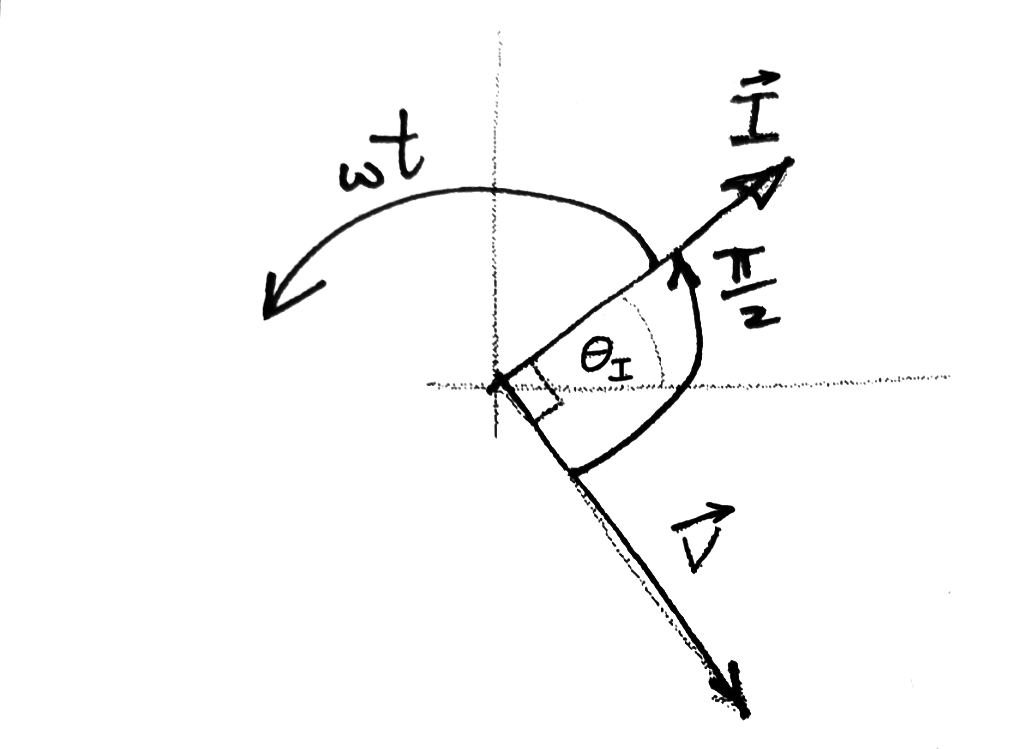
\includegraphics[width=0.35\textwidth]{figsChapt02/GM66229.png}



\subsection{Inductor}
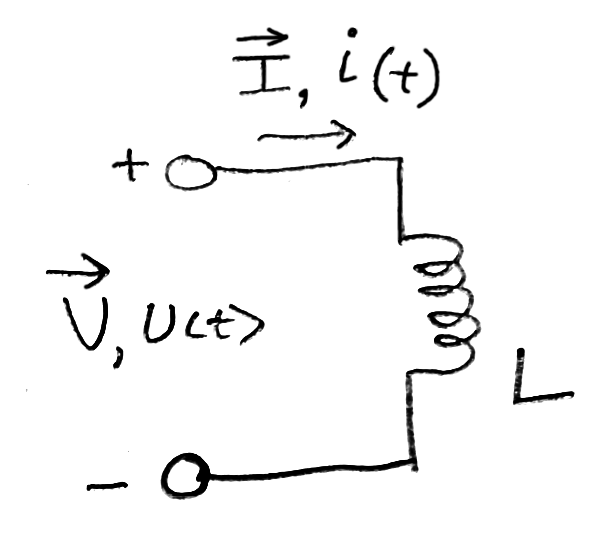
\includegraphics[width=0.35\textwidth]{figsChapt02/MP46579.png}

The analysis for the inductor is almost identical to the capacitor derivation directly above, except the consitutive equation
for the inductor is
\[
v(t) = L\frac {d}  {dt} \; i(t)
\]
so the resulting phasor impedance  equation is
\[
\vec{V} = j\omega L \vec{I}
\]
\[
Z_L = j\omega L,;\quad
\]

\begin{enumerate}
  \item $\angle{Z_L} = +\pi/2 = +90^\circ$\\
  This means the inductor current $\vec{I}$ {\bf lags} the voltage $\vec{V}$ by $\pi/2$ radians or $90^\circ$.
  \item $|Z_L| = \omega L$\\
  The higher the steady state frequency, $\omega$, or the inductance, $I$, the higher the magnitude of the impedance (and if voltage is fixed,
  the smaller the current through the inductor.)
\end{enumerate}

The vector diagram corresponding to the capacitor diagram above is the same except that the voltage would {\bf lead} the current.


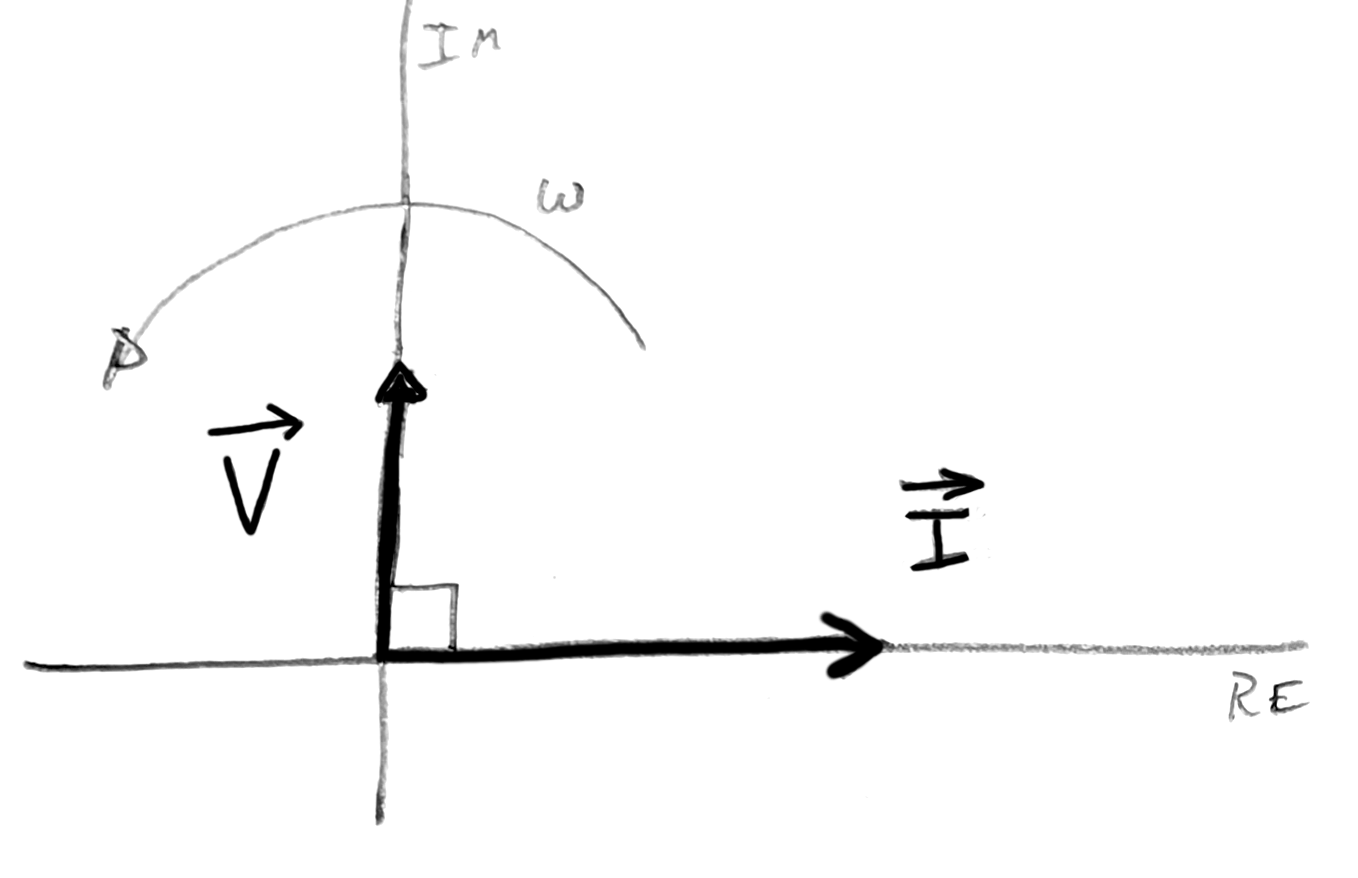
\includegraphics[width=0.35\textwidth]{figsChapt02/EC64016.png}
The resulting sinuoids can be sketched

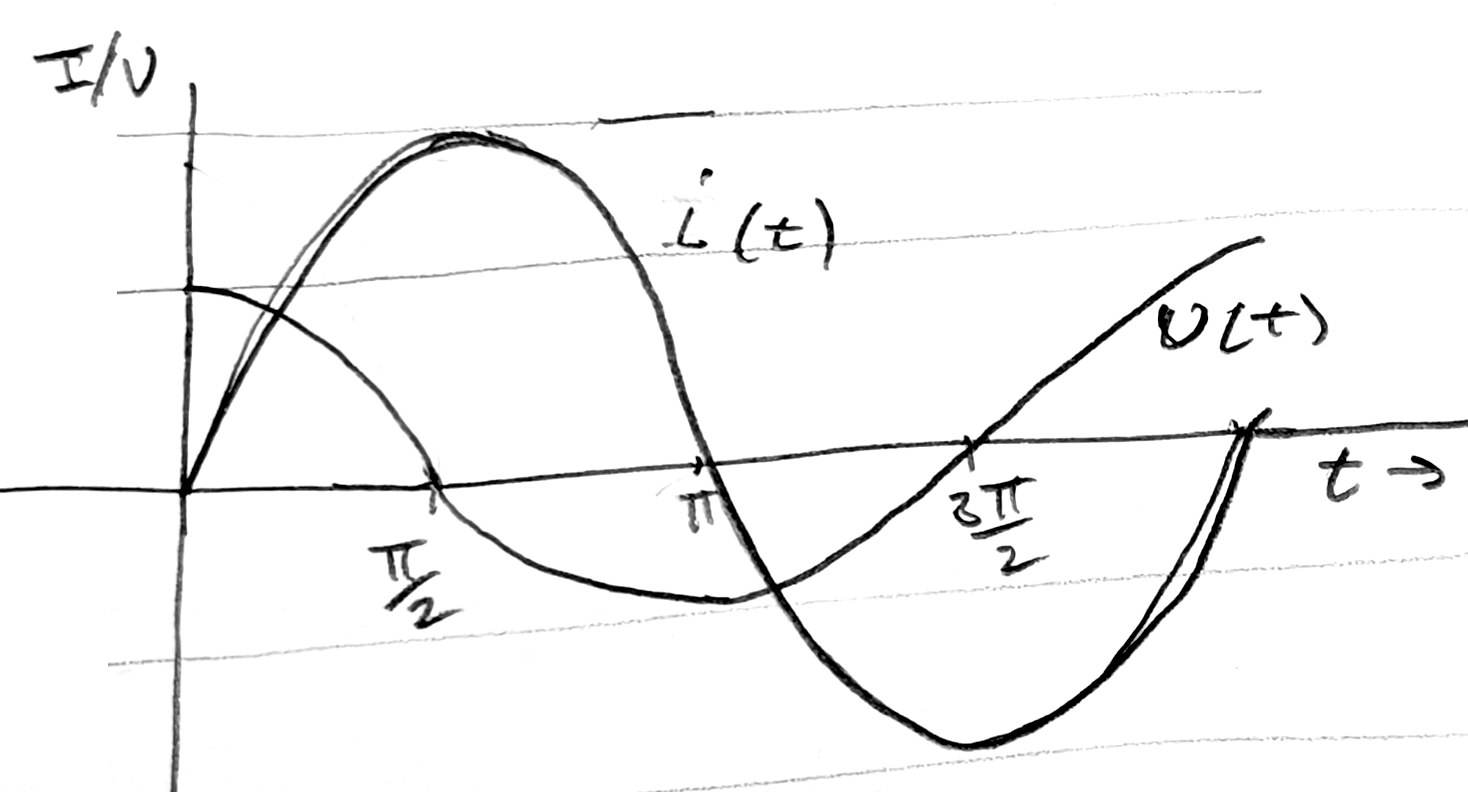
\includegraphics[width=0.35\textwidth]{figsChapt02/PP03048.png}


\section{Impedance}

We have now found complex quantities analogous to resistance for the energy storage elements, specifically

\begin{align}
\mathrm{Inductor:}  & \vec{V} = j\omega L \vec{I}\\
\mathrm{Capacitor:}  & \vec{V} = \frac{1}{j\omega C} \vec{I}\\
\end{align}
We also then have:
\[
\vec{V} = Z\vec{I}
\]
were
\[
Z = \frac {\vec{V}}  {\vec{I}}
\]
$Z$ is called ``complex impedance'' or simply ``impedance''.

We also define:
\[
\mathrm{Re}\left\{ Z\right\} = \mathrm{Resistance, ~R}
\]
\[
\mathrm{Im}\left\{ Z\right\} = \mathrm{Reactance, ~X}
\]
(note that 'R' was already taken when they had to abbreviate ``Reactance''!).

Reactance has two ``flavors'' based on it's sign.   Because
\[
X_C = \frac {-1}  {\omega C}
\]
and $\omega, C$ are always positive, we call any $X<0$ ``Capacitive Reactance''. Similarly
we call $X>0$ ``Inductive reactance'' since
\[
X_L = \omega L
\]
which is also always positive.


\subsection{Recap:}
Complex impedance, $Z$, is defined in terms of the phasors, $\vec{I}, \vec{V}$ as:
\[
Z = \frac {\vec{V}}  {\vec{I}}
\]
For inductance and capacitance, we have
\[
Z_L = j\omega L,\;\; Z_C = \frac {1}  {j\omega C}
\]
We introduced another new term, ``Reactance'', $X$, which is the imaginary part of $Z$.
\[
Z = R + jX
\]

For inductors and
capacitors, the reactances are:
\[
X_L = \omega L\;(\angle{Z_L} = \pi/2),\;\; X_C = -\frac {1}  {\omega C}\; (\angle{Z_C} = -\pi/2)
\]

\subsection{Related quantities: Admittance, Conductance, Susceptance}

\paragraph{Admittance}
Just as Conductance is $1/R$, we define Admittance, $Y$, as a complex number
which is the inverse of Impedance
\[
Y = \frac {1}  {Z} = \frac{1}{R+jX} = G+jB
\]
Note that you can derive that
\[
Y = \frac {R-jX}  {|Z|^2}
\]
(try it using properties of complex numbers).


\paragraph{Conductance and Susceptance}

The new letters in the complex value of Admittance are
\begin{align}
\mathrm{G} &= \mathrm{Re}\left \{ Y \right \} = \mathrm{Conductance}\\
\mathrm{B} &= \mathrm{Im}\left \{ Y \right \} = \mathrm{Susceptance}
\end{align}
(Note that unless $B=0$, $G \neq 1/R$!)


\subsection{}






\section{Using Phasors in Circuit Analysis }




\subsection{Series and Parallel Impedances}

Nicely, these work exactly the same as resistances:

\paragraph{Series Combinations}
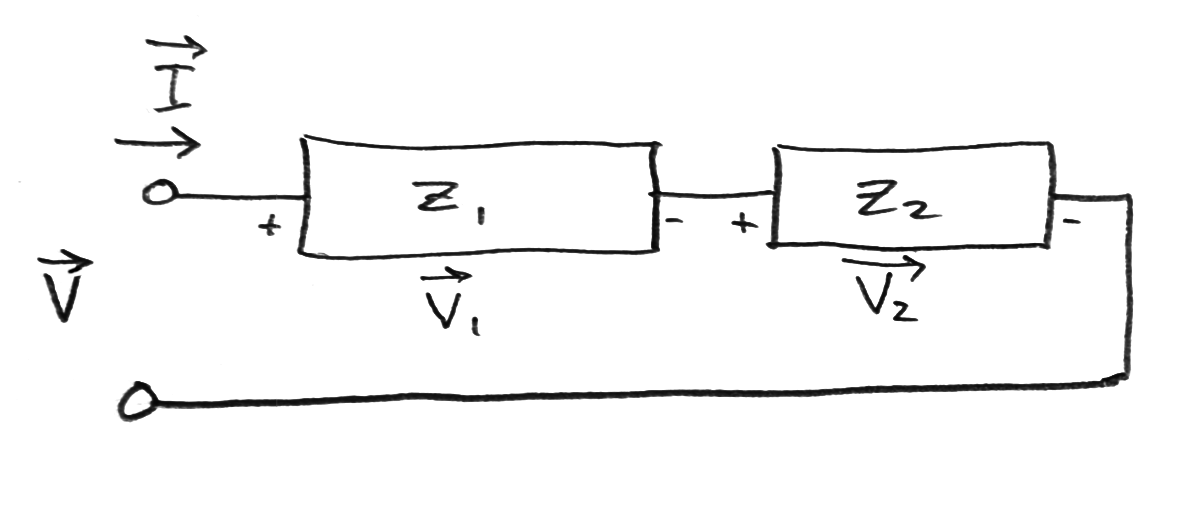
\includegraphics[width=0.3\textwidth]{figsChapt02/FT71566.png}

\[
\vec{V} = \vec{V}_1  + \vec{V}_2
\]
\[
\vec{V} = Z_1\vec{I}  + Z_2\vec{I} = \vec{I}(Z_1+Z_2)
\]
So series impedances combine by addition.

\paragraph{Parallel Combinations}
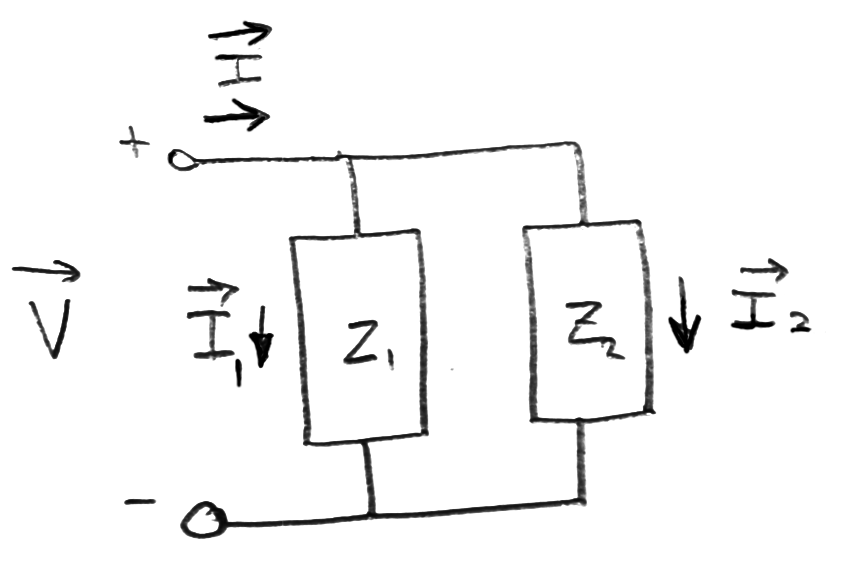
\includegraphics[width=0.3\textwidth]{figsChapt02/IM00849.png}

\[
\vec{V} = \vec{I}_1 Z_1 =  \vec{I}_2 Z_2
\]
\[
\vec{I} = \vec{I}_1 +  \vec{I}_2
\]
\[
Z_{tot} = \frac {\vec{V}}  {\vec{I}}
= \frac {\vec{V}}  {\frac {\vec{V}}  {Z_1} + \frac {\vec{V}}  {Z_2} }
\]
\[
Z_{tot} = \frac {1}  {\frac {1}  {Z_1}  + \frac {1}  {Z_2}  }
\]

Parallel impedances combine like parallel resistances:
\[
Z_{par} = \frac {1}  {\sum\limits_{i} \frac {1}  {Z_i} }
\]





\section{Circuit Examples}


\subsection{RL Circuit}\label{seriesRLckt}

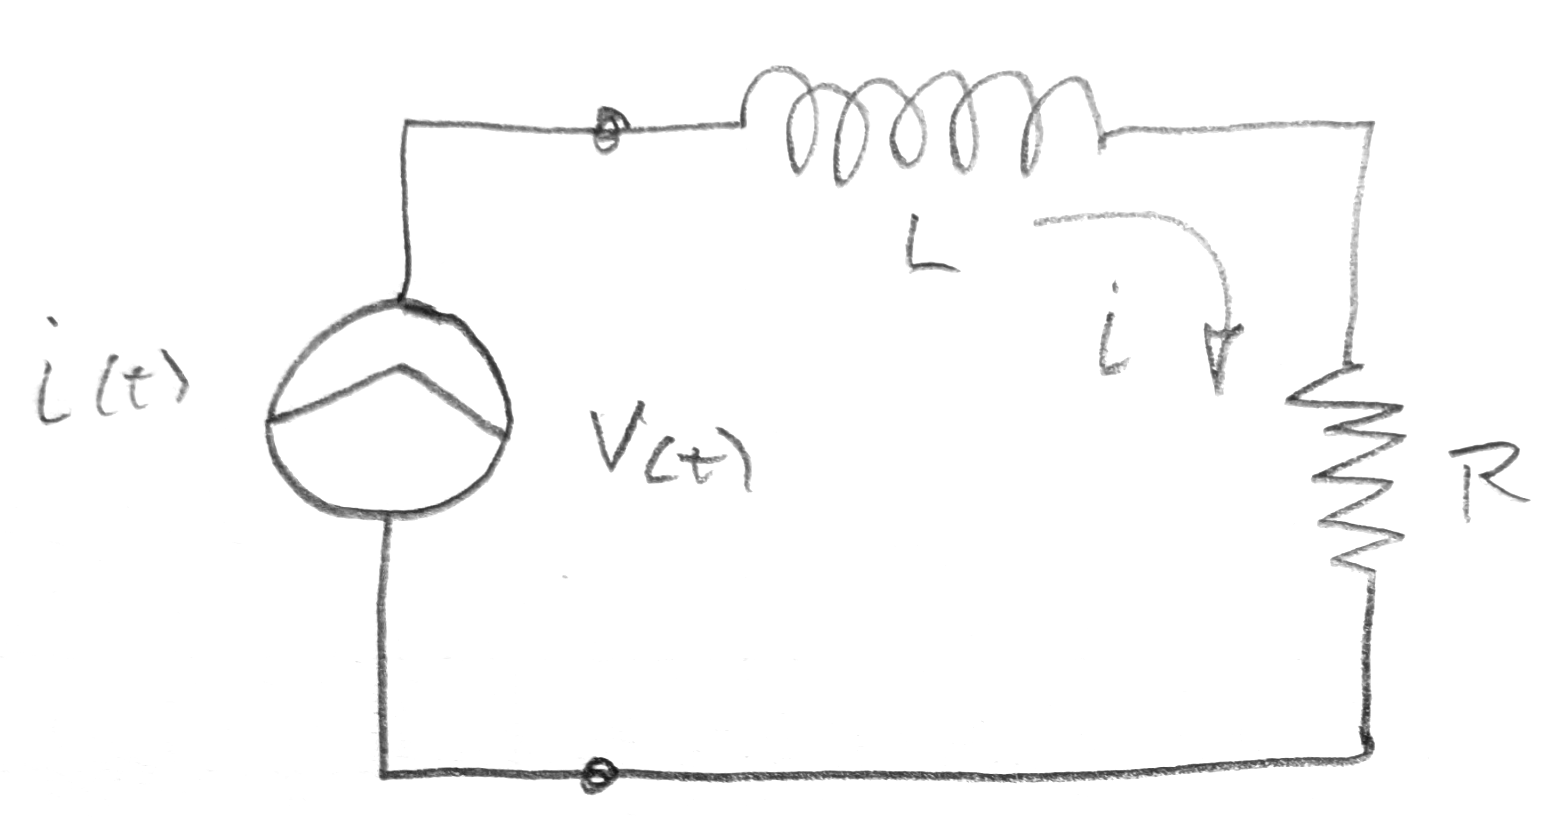
\includegraphics[width=0.5\textwidth]{figsChapt02/RI98726.png}

\paragraph{Problem:} Find $\vec{V}$ and $v(t)$ by the phasor method.
\paragraph{Solution:}
Deriving the current phasor:
\[
i(t) = I_M\cos(\omega t),\;\; \vec{X} = I_Me^{j0} = I_M
\]

1)
Evaluate phasor voltage drops and combine them via KVL
\[
\vec{V} = j\omega L \vec{X} + \vec{X} R
\]

2) Solve for $\vec{V}$:
\[
\vec{V} = \vec{X} (R+j\omega L)
\]
\[
\vec{V} = I_MR + jI_M \omega L
\]
\[
|\vec{V}| = \sqrt{I_M^2 R^2 + I_M^2(\omega L)^2} \equiv V_M = I_M\sqrt{R^2+(\omega L)^2}
\]
\[
\angle{\vec{V}} = \tan^{-1}(\frac {\omega L}  {R} ) \equiv \theta
\]
\[
\vec{V} = V_Me^{j\theta}
\]

note  $\vec{V} = \vec{X}(R+j\omega L) $ is just like Ohms Law, $V=IR$ if that $R$ were complex.

Since the complex reactances have their own directions (in the complex plane), we can diagram the summation


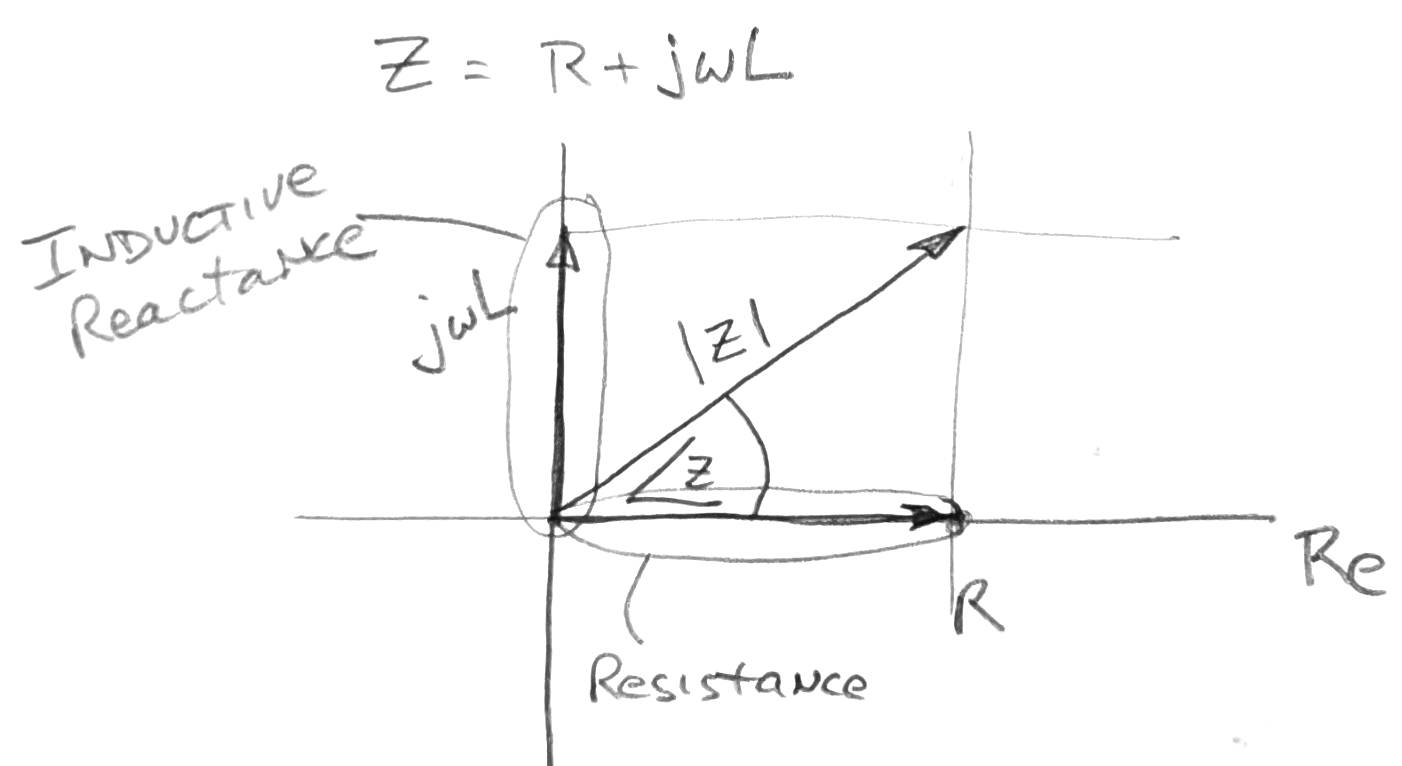
\includegraphics[width=0.5\textwidth]{figsChapt02/UI87197.png}

The imaginary part of the impedance is $j\omega L$, and the real part is $R$.
If we also had a capcitor in the circuit, it would have a negative (aka ``capacitive") reactance,
and the diagram would look like

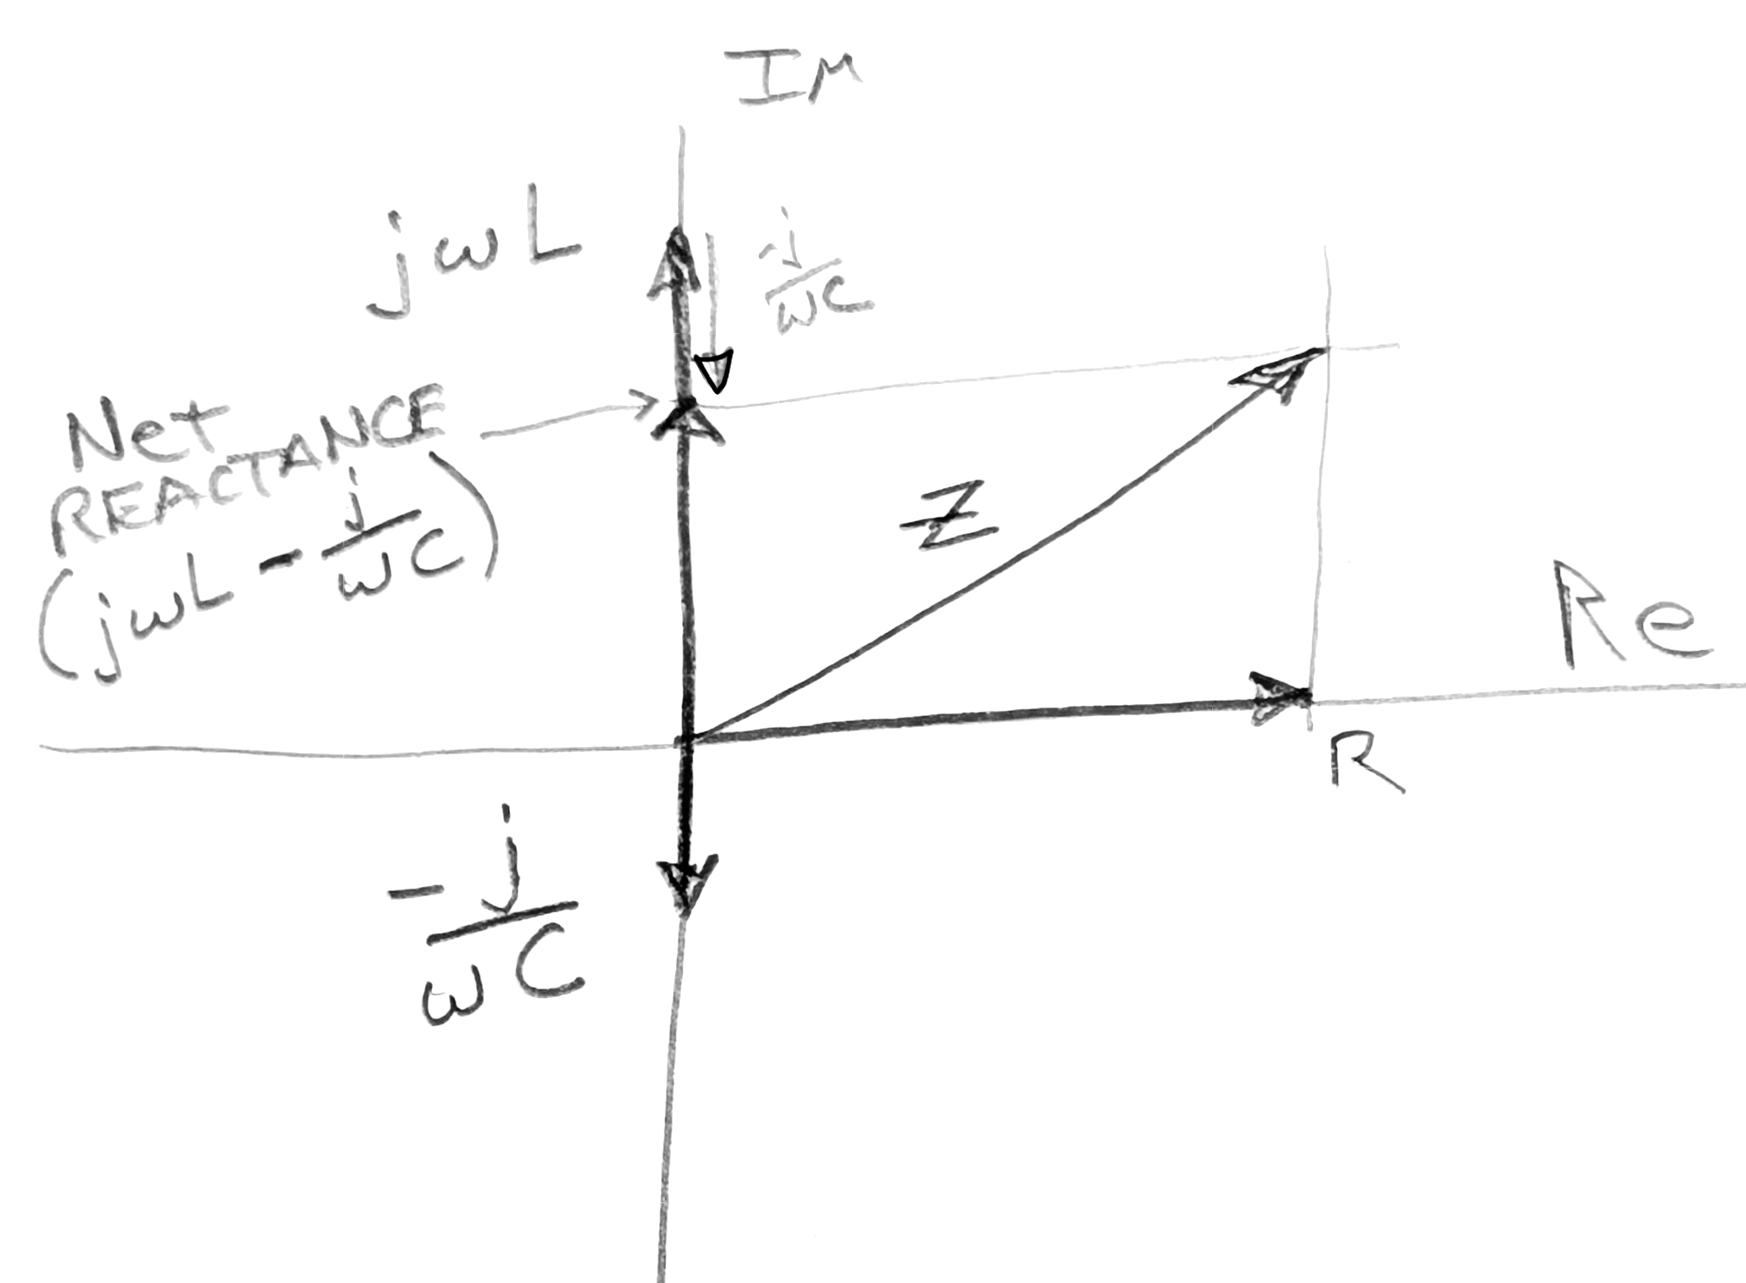
\includegraphics[width=0.5\textwidth]{figsChapt02/HF41781.png}

\subsection{More complex circuit}

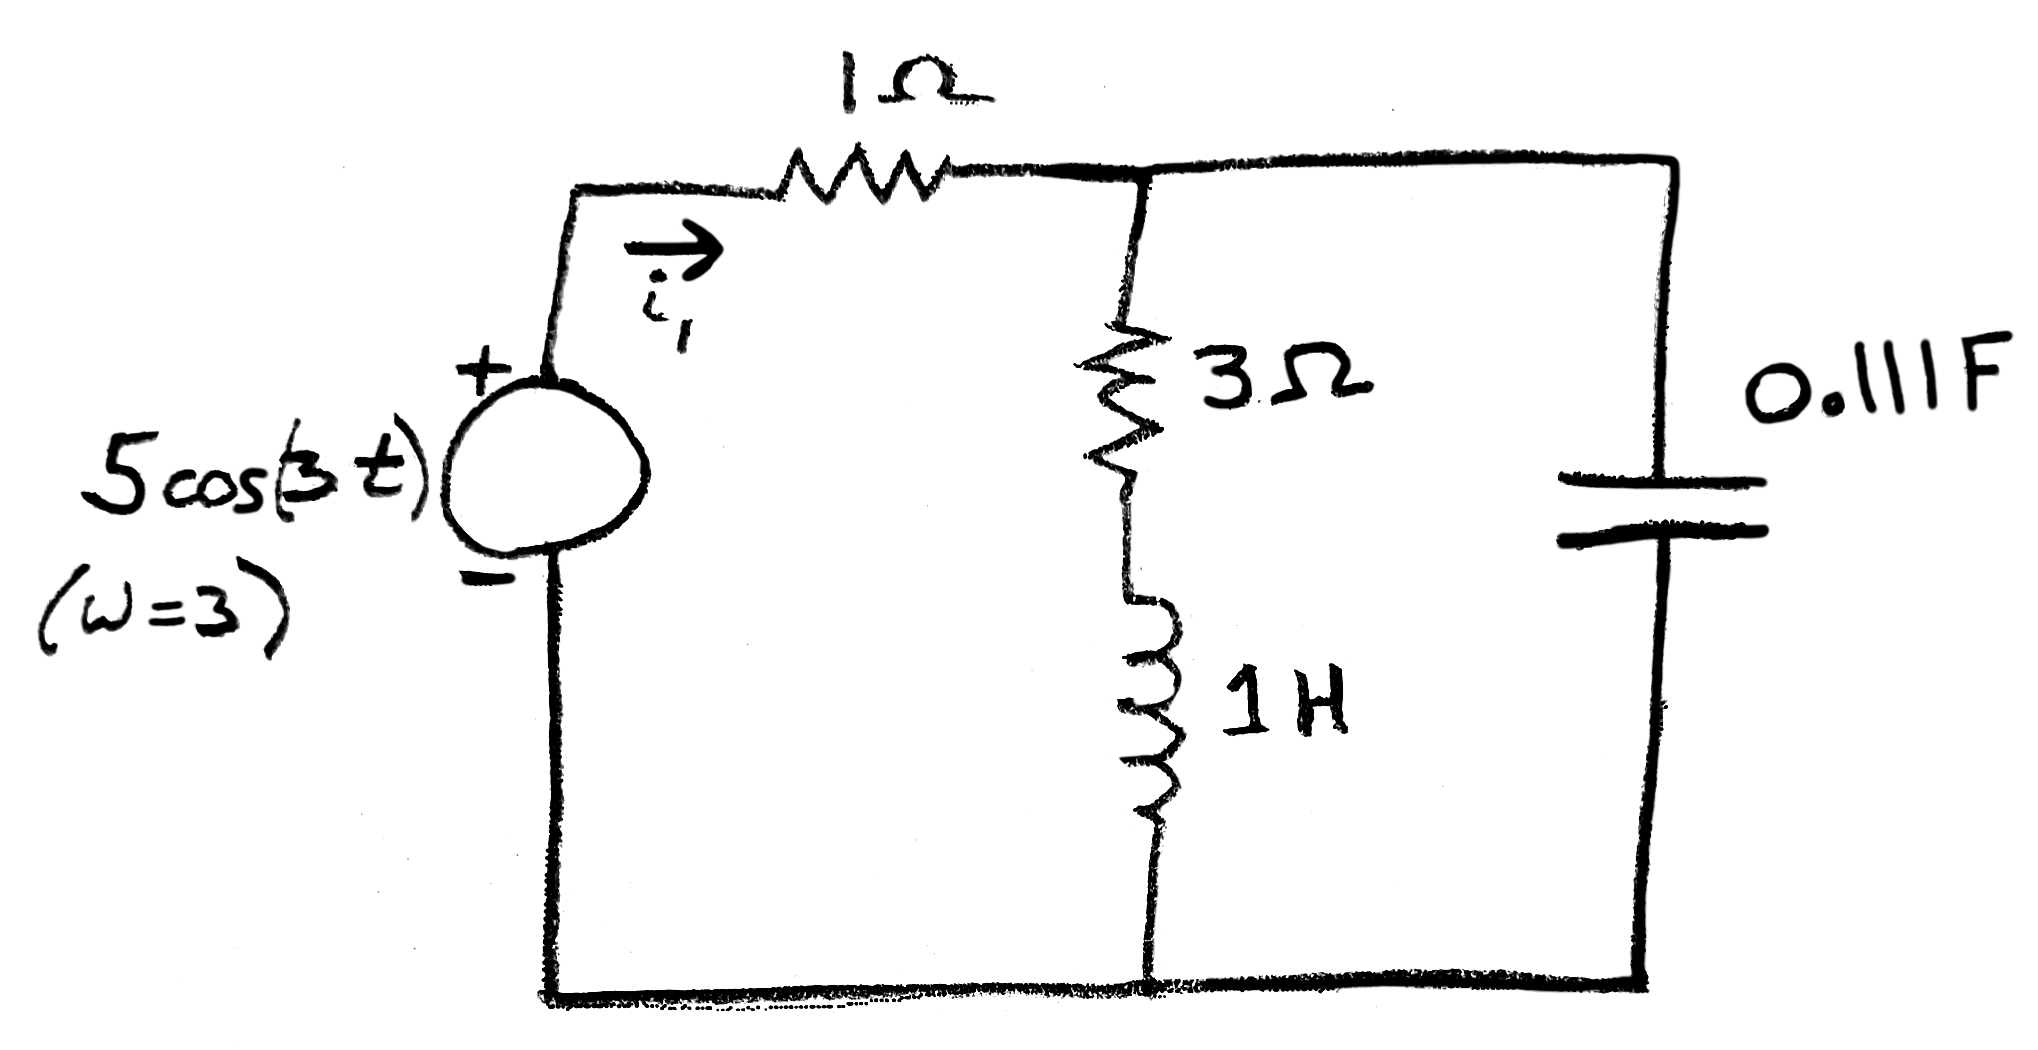
\includegraphics[width=0.5\textwidth]{figsChapt02/AM06622.png}

Q: Find the sinusoidal  steady state value of $i_1(t)$

A:

\[
\vec{I} = \frac{\vec{V}}  {Z} \; \to\; Z = \frac {\vec{V}}  {\vec{I}}
\]

Evaluate the impedances  in-place:

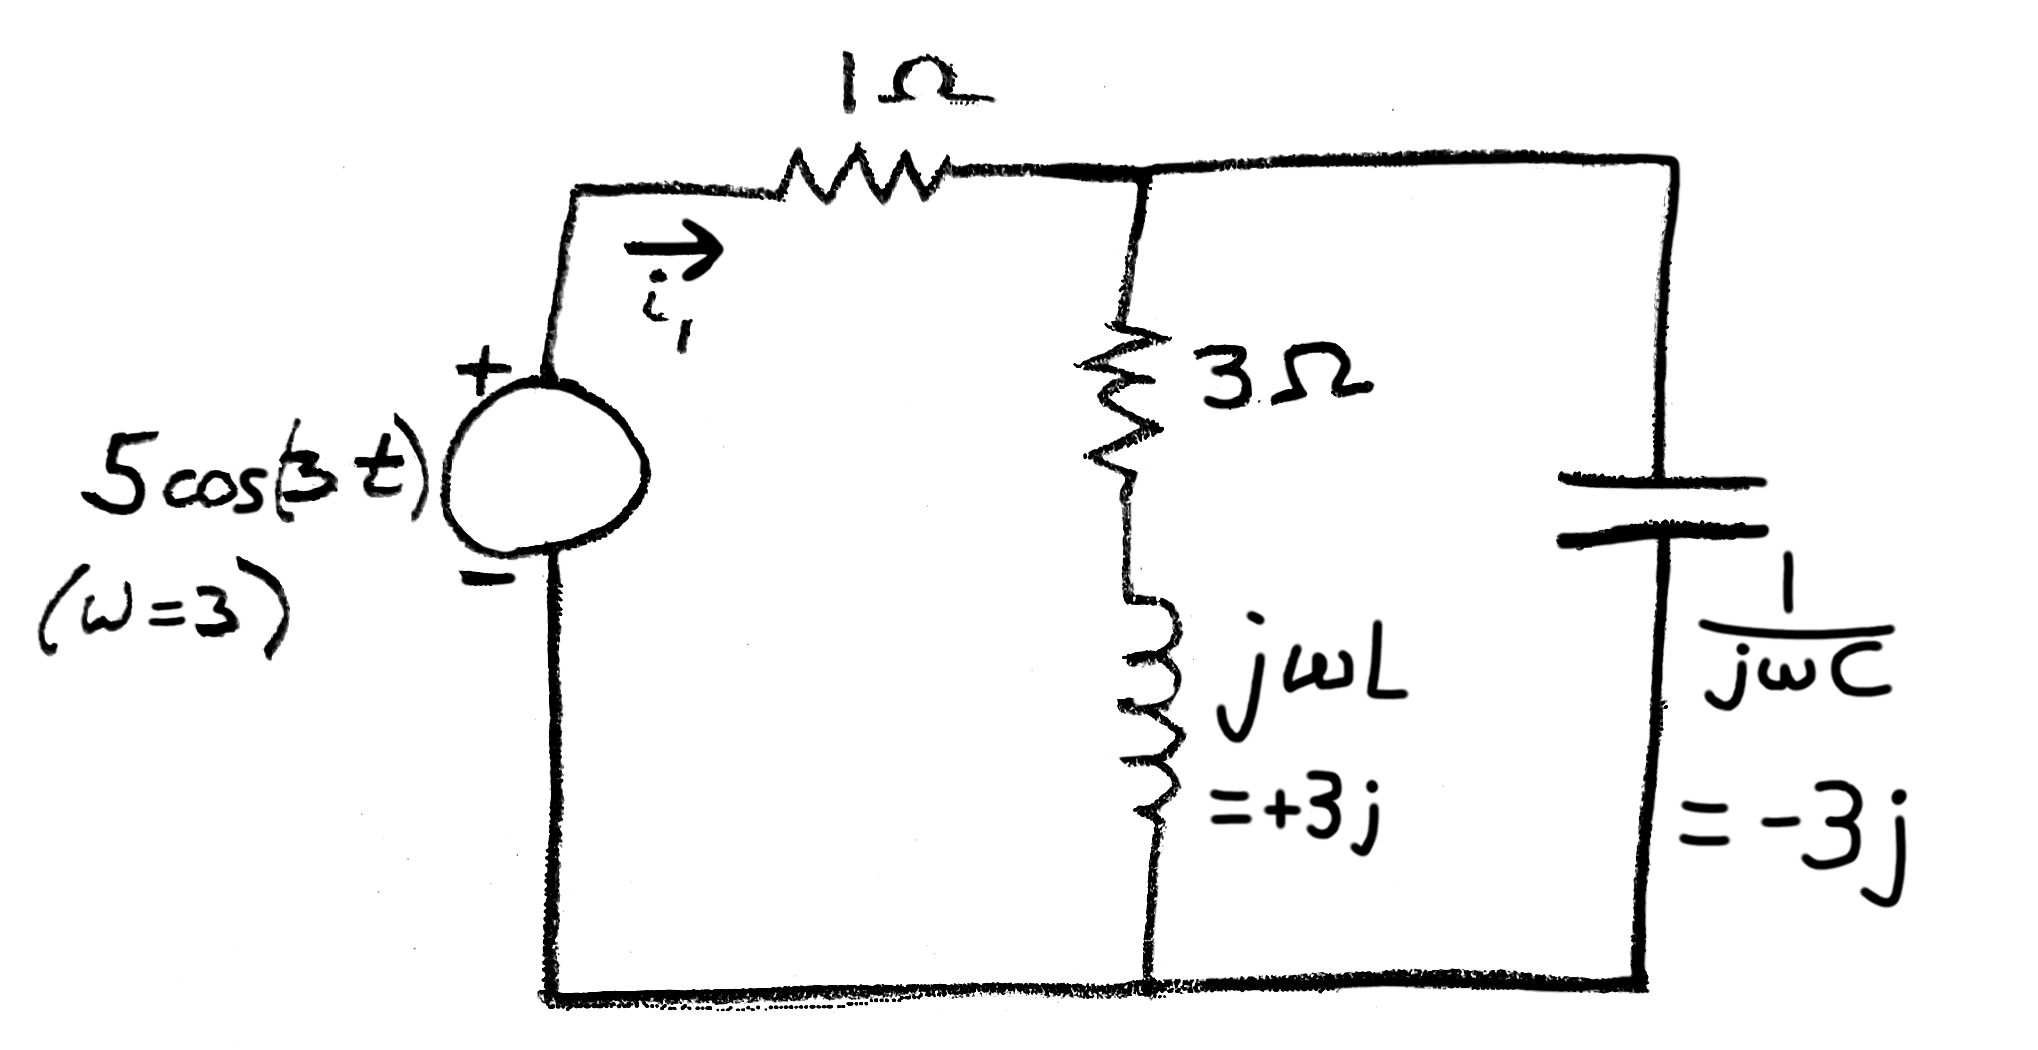
\includegraphics[width=0.5\textwidth]{figsChapt02/ME02007.png}

\[
Z =  1 + \frac{(3 + j3)(j3)}{3 + j3 + j3} = 1 + \frac{9 - 9j}{3} = 1 + 3 - 3j
= 4 - 3j
\]
(Net reactance is negative in other words, Capacitive)

\[
|Z| = \sqrt{16 + 9} = 5\Omega
\]


\[
\angle Z = \tan^{-1}\left(\frac{-3}{4}\right) = -37^\circ
\]

\[
\vec{I} = \frac{\vec{V}}{Z} = \frac{5e^{j0t}}{5e^{j37^\circ}} = 1e^{j37^\circ}
\]

\[\boxed{
i_L(t) = 1\cos(3t + 37^\circ)
}\]




Let's do one more KVL circuit example, just like Example \thechapter.\ref{firstPhasorCktKVL}, but with the addition of a capacitor.


\subsection{Series RLC  Circuit}\label{2ndPhasorCktKVL}

Now we add a capacitor to the simple series RL circuit:

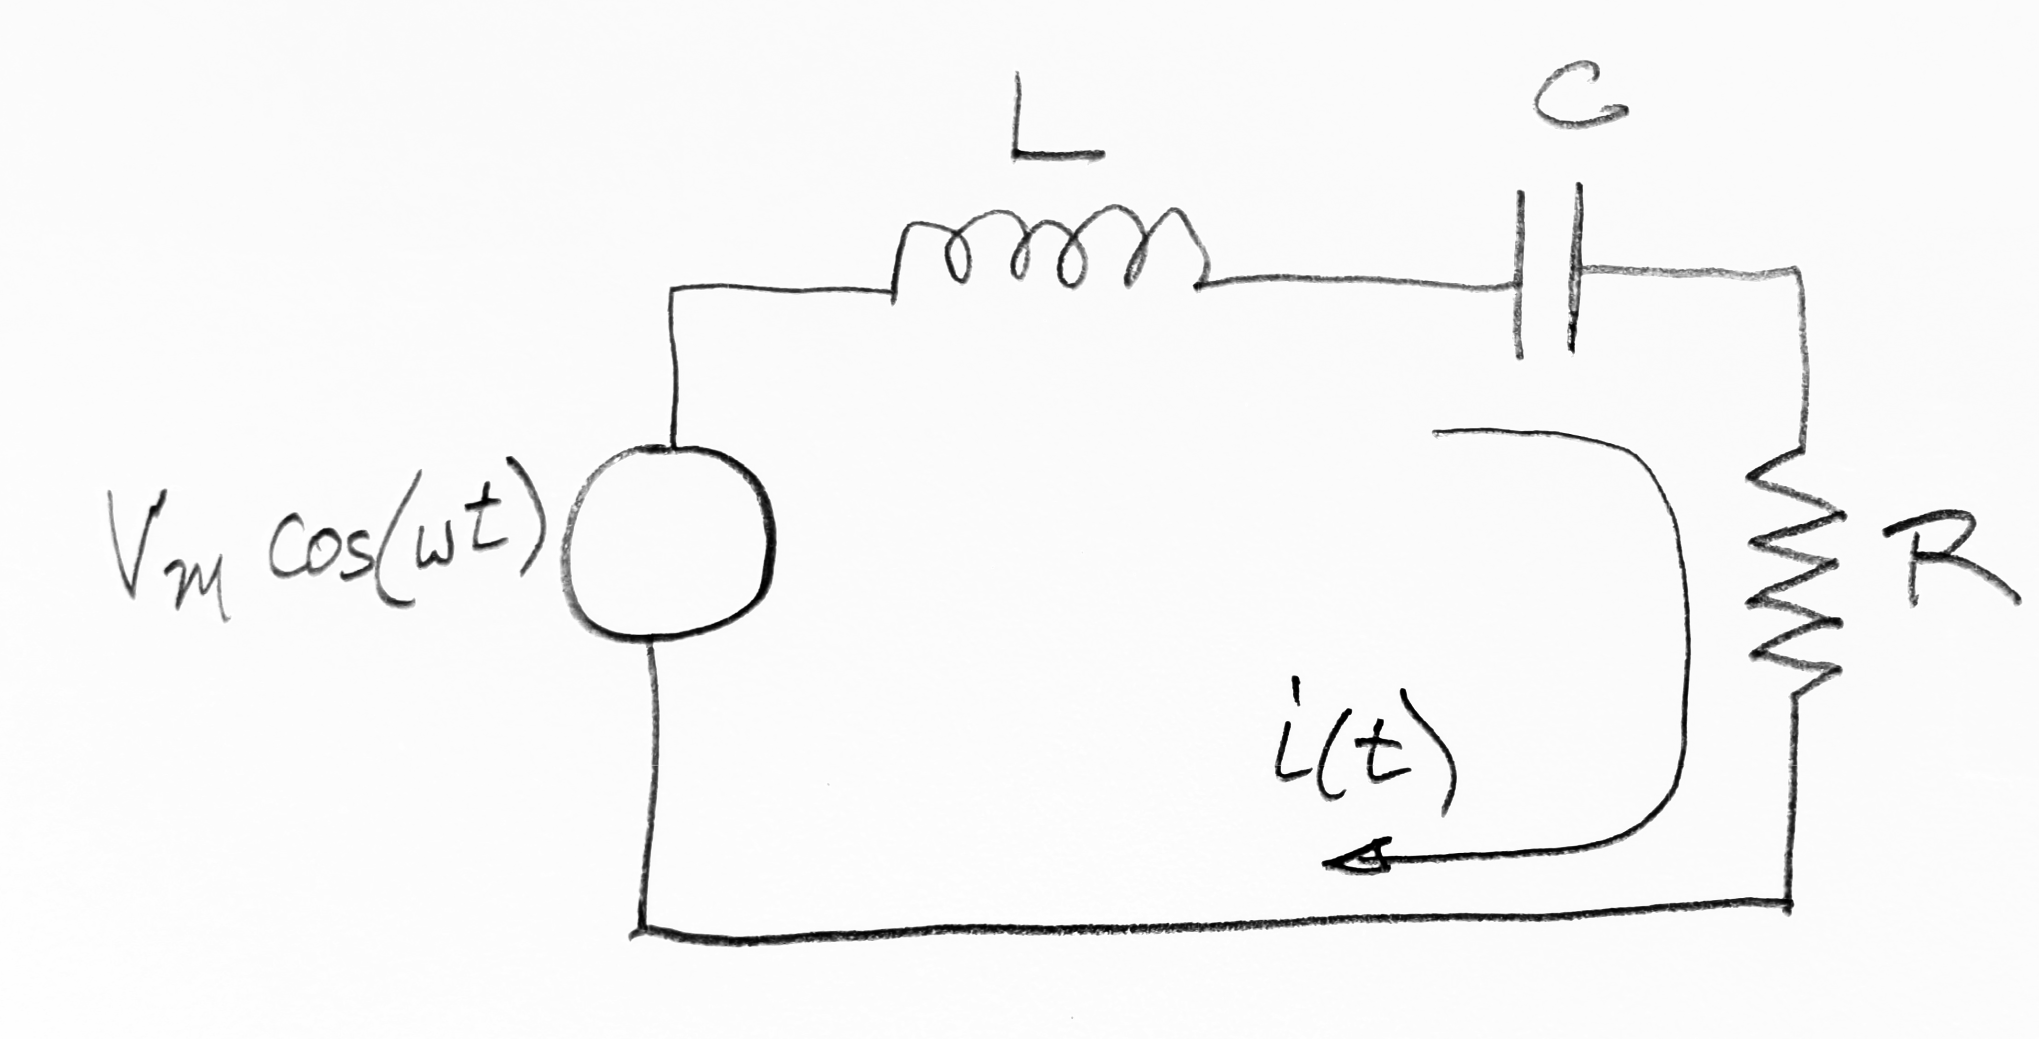
\includegraphics[width=0.5\textwidth]{figsChapt02/EL44497.png}

\begin{enumerate}
\item Using the definitions of capacitors, inductors, and resistors, and summing the  voltages around the loop:

\[
-V_M\cos(\omega t) + L\frac{di}{dt} + \frac {1}  { C}\int_0^t i\; dt + iR = 0
\]

\[
V_M\cos(\omega t) = L\frac{di}{dt}  + \frac {1}  {C}\int_0^t i\; dt + iR
\]

\item Consider input voltage to be the real part of two complex sinusoids:

\[
V_M\cos(\omega t) = \mathrm{Re}\{ \vec{V}e^{j\omega t} \}
\]
And we define
\[
i(t) = \mathrm{Re}\{ \vec{I}e^{j\omega t}  \}
\]
as the current phasor which is
unknown.

% \noindent $\{i \cdot \vec{V}, \vec{I}, V_0\}$

\item We plug the unknown current and voltage phasors into (1)

\[
\vec{V}e^{j\omega t} = j\omega L\vec{I}e^{j\omega t} + \frac {1}  {j\omega C}\vec{I}e^{j\omega t} +  R\vec{I}e^{j\omega t}
\]
(the leading $j\omega L$ term on the RHS comes from differentiating as in the original LODE and the $\frac {1}  {j\omega C}$
term comes from integration).


\item Next we factor out and cancel $e^{j\omega t}$ from all the terms:
\[
\vec{V} = j\omega L\vec{I} + \frac{1}{j\omega C} \vec I + R\vec{I}  = \vec{X}(R + j\omega L)
\]

As before we assume zero phase angle for input sinusoids so in this (common) case we have
\[
\vec{V} =V_Me^{j0} = V_M
\]


\end{enumerate}




Looking back at Section \ref{2ndPhasorCktKVL}, we get an abbreviated KVL analysis procedure.

First, we plugged in phasors for the sinusoidal quantities and
we got:

\[
\vec{V}e^{j\omega t} = j\omega L\vec{I}e^{j\omega t} + \frac{1}{j\omega C}\vec{I}e^{j\omega t} + \vec{I}Re^{j\omega t}
\]

Next we can  cancel out $e^{j\omega t}$ from every term giving

\[
\vec{V}  = j\omega L\vec{I}  + \frac{1}{j\omega C}\vec{I}  + \vec{I}R
\]
Now let's factor out $\vec{I}$ from all the RHS terms which gives

\[
\vec{V} = \vec{I} \left( j\omega L + \frac {1}  {j\omega C} +   R \right)
\]

The key observation is that we now are multiplying $\vec{I}$ by a single complex number to get $\vec{V}$
--- {\it instead of solving a differential equation!}


We call this complex quantity, in this circuit  $j\omega L + \frac {1}  {j\omega C} +   R $,
the Complex Impedance, or simply {\bf Impedance} of the circuit.
It is analogous to resistance, but   for sinusoidal
steady state problems.
So for this important class of AC problems, we can use a complex version of Ohm's law just
like DC circuits!


\begin{ExampleSmall}
Continue solving Example \ref{2ndPhasorCktKVL} to get the current phasor
$\vec{I}$.

\paragraph{Solution}

\[
\vec{I} = \frac {\vec{V}}  {j\omega L + \frac {1}  {j\omega C} +   R} =
\frac {V_M}  {j\omega L + \frac {1}  {j\omega C} +   R}
\]

($\vec{V} =V_M$
because we usually choose the source voltage to have zero phase,
$\vec{V} = V_Me^{j\omega t + 0}$
).

Simplifying we multiply by $j/j$:
\[
= \frac {jV_M}  {-\omega L + \frac {1}  {\omega C} + jR }
\]
\[
\vec{I} = \frac {jV_M}  {(\frac {1}  {\omega C}-\omega L) + Rj} = \frac {V_M}  {R-j(\frac {1}  {\omega C}-\omega L)}
\]
dividing complex numbers is easier in polar form so
\[
|R-j(\frac {1}  {\omega C}-\omega L)| = \sqrt{R^2+ \left (\frac {1}  {\omega C}-\omega L\right )^2}
\]
\[
\angle{R-j\left (\frac {1}  {\omega C}-\omega L\right )}  = -\tan^{-1}\left ( \frac {\frac {1}  {\omega C}-\omega L}  {R} \right )
\]
\[
\vec{I} = V_M \frac {1}  {\sqrt{R^2+(\frac {1}  {\omega C}-\omega L)^2}}e^{j\phi},\;\; \phi =  -\tan^{-1}\left ( \frac {\frac {1}  {\omega C}-\omega L}  {R} \right )
\]
\end{ExampleSmall}



\subsection{Effects of Frequency on Reactance}

Looking again at the impedance of the circuit in the previous subsection, we have
\[
Z_{tot}  =  j\omega L + \frac {1}  {j\omega C} +   R
\]

Diagramming the impedance components as we did in section \ref{seriesRLckt}, we see that
the inductive reactance and the capacitive reactance are always in opposition.  Repeating
the diagram:

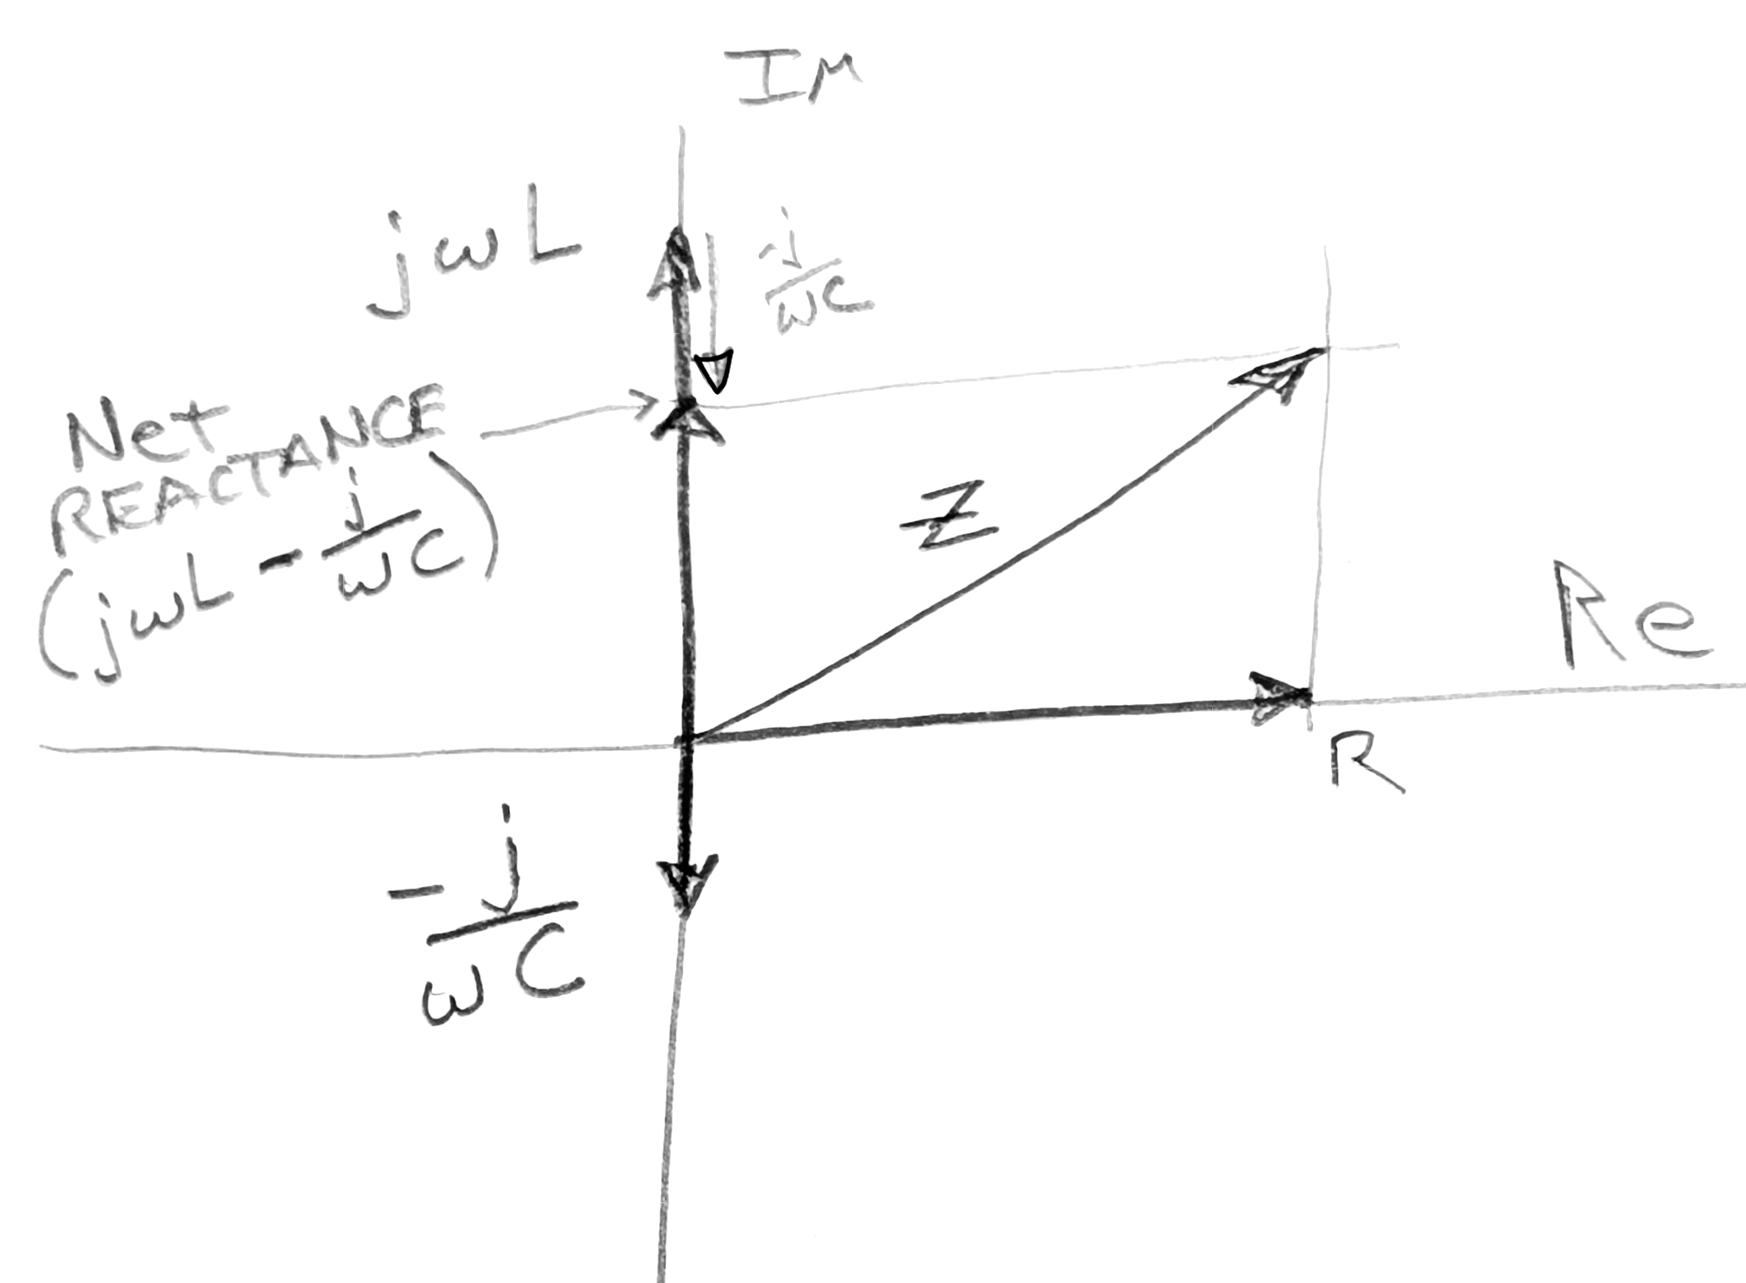
\includegraphics[width=0.5\textwidth]{figsChapt02/HF41781.png}

Notice that $\omega$ appears inverted in the capacitive reactance, so the magnitude of these
two components varies inversely with frequency.

Let's compute the net reactance for a series of frequencies. Where
\[
Z_{2}  =  j\omega L + \frac {1}  {j\omega C}
\]
(only the imaginary components of $Z_{tot}$).
Of course we have to assume some component values:

eg.
\[
L = 1\text{mH},\; C = 1000\mu\text{F}
\]

Writing a tiny python script to
chart the reactance ($X$) at several frequencies we get:

\begin{verbatim}import numpy as np
L = 0.001
C = 1.0E-3
j = 0.0+1.0j
ww = [10, 100, 5E2, 1000, 5e3, 1.0e4, 1.0e5]
print(' w             X')
for w in ww:
   X = j*w*L + 1.0/(j*w*C)
   print(f'{w:.2e} {np.imag(X):>8.2f}')

 w             X
1.00e+01   -99.99
1.00e+02    -9.90
5.00e+02    -1.50
1.00e+03     0.00
5.00e+03     4.80
1.00e+04     9.90
1.00e+05    99.99
\end{verbatim}

For these component values the net reactance is negative (capacitive) below 1000 rad/sec
and positive (inductive) above 1000 rad/sec.

Let's take this one step further and evaluate the whole impedance (putting $R$ back in the picture).
We have to specify the resistance:
\[
R = 10\Omega
\]
Now the script changes to

\begin{verbatim}import numpy as np
L = 0.001
C = 1.0E-3
R = 10
j = 0.0+1.0j
ww = [ 10, 100, 5E2, 1000, 5e3, 1.0e4, 1.0e5]
print(' w             X      |Z|        /_Z (deg)       Z')
for w in ww:
   X = j*w*L + 1.0/(j*w*C)
   Z =  R + j*w*L + 1.0/(j*w*C)
   ang = 360 * np.angle(Z)/(2*np.pi)
   print(f'{w:.2e} {np.imag(X):>8.2f}  {np.abs(Z):>8.2f}  {ang:>8.2f}
            {np.real(Z):8.2f} + {np.imag(Z):8.2f}j' )

 w             X      |Z|        /_Z (deg)       Z
1.00e+01   -99.99    100.49    -84.29      10.00 +   -99.99j
1.00e+02    -9.90     14.07    -44.71      10.00 +    -9.90j
5.00e+02    -1.50     10.11     -8.53      10.00 +    -1.50j
1.00e+03     0.00     10.00      0.00      10.00 +     0.00j
5.00e+03     4.80     11.09     25.64      10.00 +     4.80j
1.00e+04     9.90     14.07     44.71      10.00 +     9.90j
1.00e+05    99.99    100.49     84.29      10.00 +    99.99j
\end{verbatim}

Note how the angle changes to almost $\pm90^\circ$ as the magnitude of the reactance dominates $R$.

\section{Voltage and Current Dividers with Impedances}
Just as with parallel and series combinations, voltage dividers work in a very similar way with impedances.


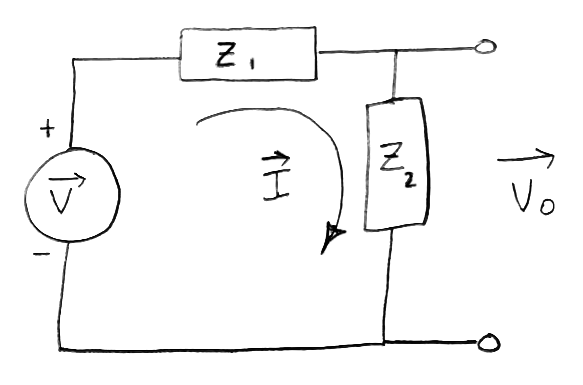
\includegraphics[width=0.35\textwidth]{figsChapt02/CT64010.png}

\[
\vec{V} = \vec{I}(Z_1+Z_2)
\]
\[
\vec{V}_o = \vec{I} Z_2
\]
\[
\frac {\vec{V}_0 } {\vec{V}} = \frac {Z_1}  {Z_1+Z_2}
\]

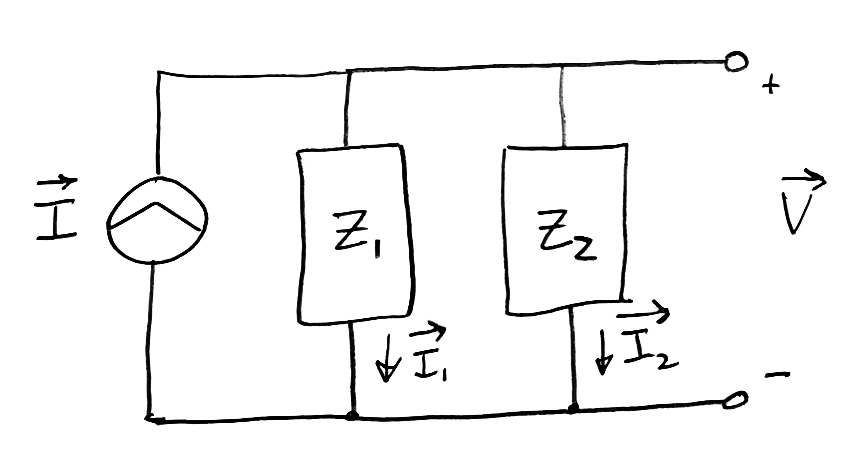
\includegraphics[width=0.35\textwidth]{figsChapt02/LE10258.png}

For Current Dividers, we can leverage admittances, which like conductances, make it somewhat simpler.
\[
\vec{I} = \vec{V}(Y_1+Y_2) = \vec{V}(\frac {1}  {Z_1} + \frac {1}  {Z_2}  )
\]

\[
\vec{I}_1 = \vec{V} Y_{1}
\]

\[
\frac {\vec{I}_1}  {\vec I_1+\vec I_2} = \frac {\vec V Y_1}  {\vec V (Y_1+Y_2)}
\]

\[
\frac {\vec{I}_1}  {\vec I_1+\vec I_2} = \frac {\frac {1}  {Z_1}}  {\frac {1}  {Z_1}+\frac {1}  {Z_2}} =
\frac {1}  {1+\frac {Z_1}  {Z_2} } = \frac {Z_2} {Z_1+Z_2}
\]

And for three parallel impedances:


\[
\frac {\vec{I}_1}   {\vec I_1+\vec I_2+\vec I_3} = \frac {Y_1}  {Y_1+Y_2+Y_3} =
\frac {\frac {1}  {Z_1}}  {\frac {1}  {Z_1}+\frac {1}  {Z_2}+\frac {1}  {Z_3}} =
\frac {Z_2 Z_3}  {Z_2 Z_3 + Z_1 Z_3+ Z_1 Z_2}
\]

\section{Thevenin and Norton Equivalents with Impedances}

Consider a ``black box'' -- a circuit with (in this case) two terminals, but we can't see what's inside it.   Or, we can see
a very complex network of sources and impedances inside and we want a simpler {\it but equivalent} version.

\begin{center}
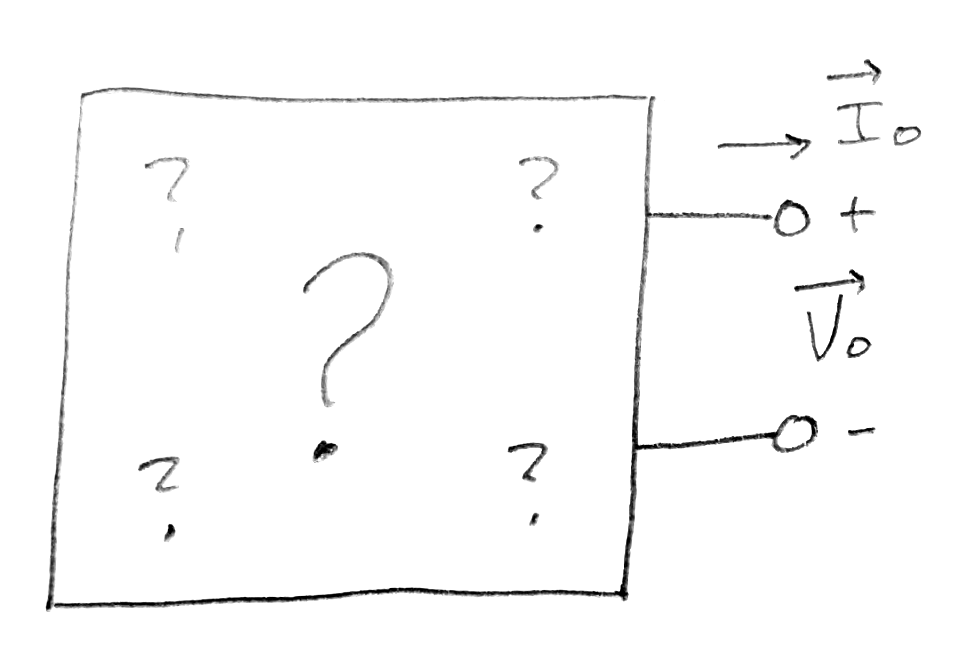
\includegraphics[width=0.25\textwidth]{figsChapt02/AJ40622.png}
\end{center}

With phasors and impedances we can redo the DC concepts of Theven and Norton equivalent circuits as follows:

\vspace{0.2in}
\noindent
\hspace{0.5in}Thevenin \hspace{2.0in} Norton

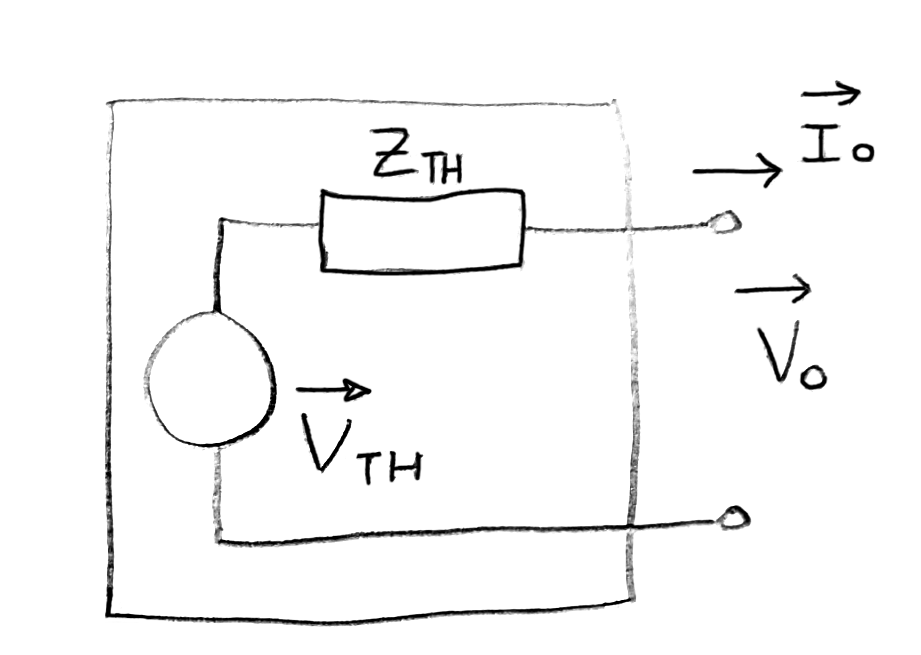
\includegraphics[width=0.25\textwidth]{figsChapt02/GT93824.png}\hspace{1.0in}
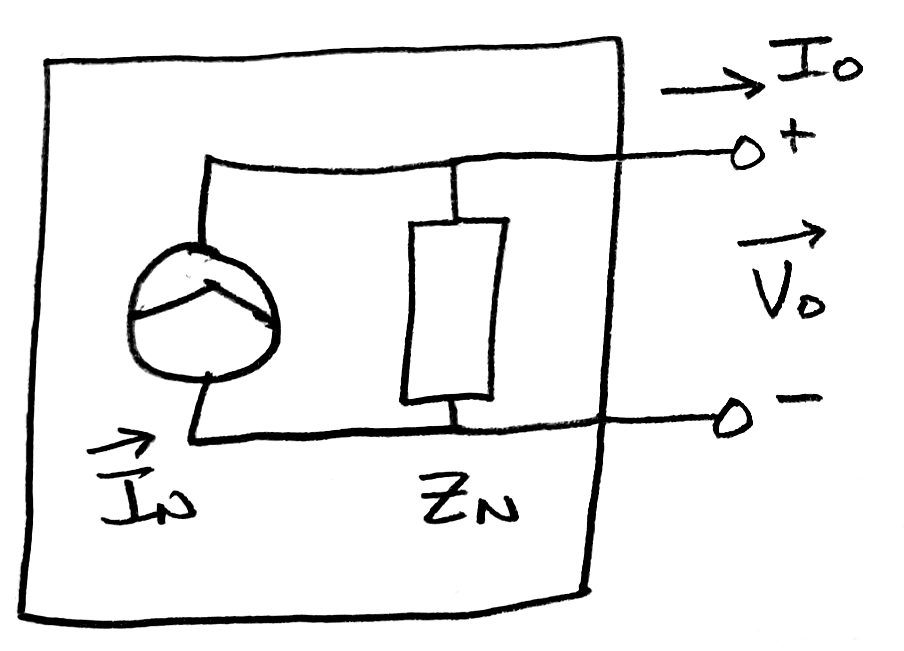
\includegraphics[width=0.25\textwidth]{figsChapt02/UN79919.png}

\vspace{0.2in}
We have a KVL equation to define the Thevenin equivalent:
\[
-\vec{V}_{TH} + \vec{I}_o Z_{TH} + \vec{V}_o = 0
\]

\[\boxed{
\vec{V}_{TH} = \left . \vec{V}_o \right |_{\vec{I}_o=0}
}
\]
(where $\vec{I}_o=0$ is the same as an open circuit of the output.)
\[\boxed{
Z_{TH} = \left . \frac
        { \vec{V}_{TH}}
        { \vec{I}_o}
        \right |_{\vec{V}_o=0  }
  }
\]
(where $\vec{V}_o=0$ is the same as a short circuit of the output.)

We also have a KCL equation to define the Norton equivalent:
\[
\vec{I}_N = \left . \vec{I}_o \right|_{\vec{V}_o=0}
\]
\[\boxed{
\vec{I}_N = \left . \vec{I}_o \right|_{\vec{V}_o=0}
}
\]
\[\boxed{
Z_N = \left . \frac {\vec{V}_o}  {\vec{I}_N} \right | _{\vec{I}_o = 0} }
\]


Note that as in the DC case, $Z_{TH} =Z_N$.


\subsection{Theven  Example with Phasors}
\begin{Example}

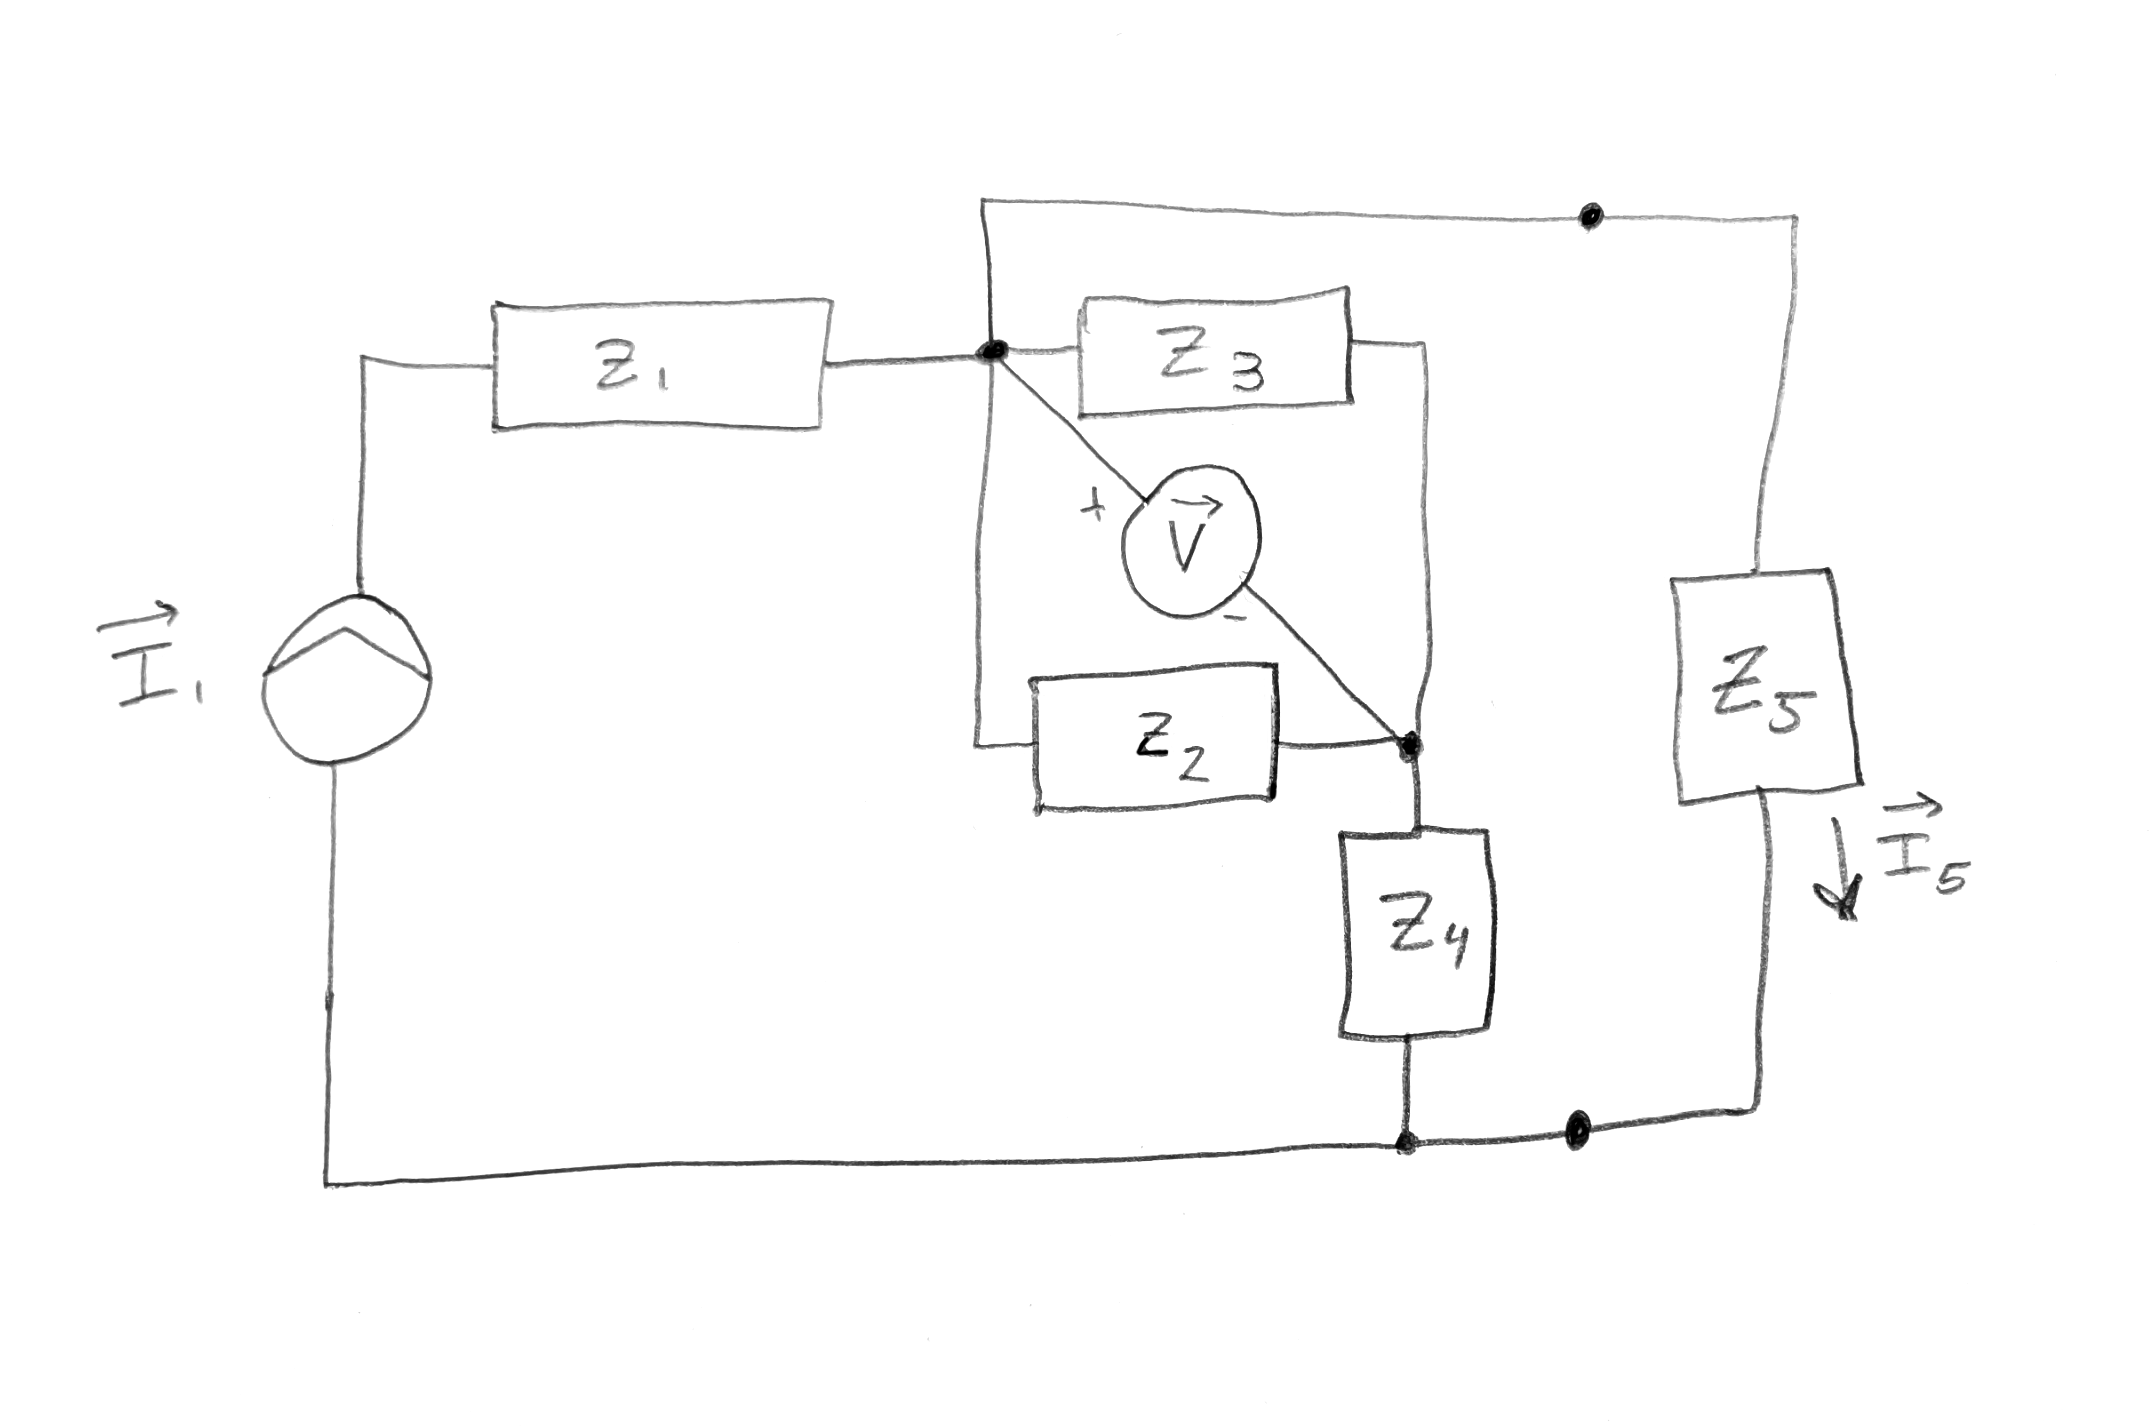
\includegraphics[width=125mm]{figsChapt02/KS52020.png}

\paragraph{Problem:} We need to find $\vec I_5$ in the above circuit. We {\it could}
write node and mesh equations, solve them, and get $\vec I_5$.

{\bf Warning:}  This is a tricky circuit!
Do not get too frustrated on this problem, give it a try and then read through the analysis
below if you get stuck!


\paragraph{Solution:}
We'll try a
Thevenin  equivalent circuit as follows.


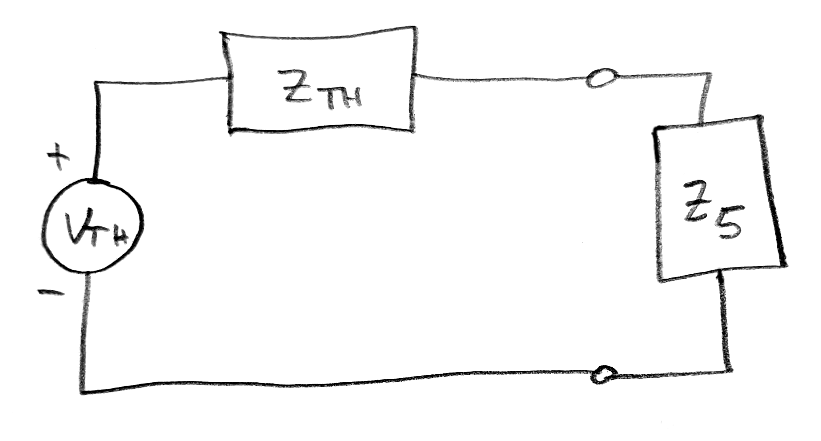
\includegraphics[width=66mm]{figsChapt02/DE22052.png}

If we can get all the stuff to the left of $Z_5$ into the Thevenin equivalent,
the problem will be simple, specifically,

\[
\vec I_5 = \frac {\vec V_{TH}}  {Z_{TH}+Z_5}
\]

We learned above that
\[
\vec{V}_{TH} = \left . \vec{V}_o \right |_{\vec{I}_o=0}
\quad
\text{and}
\quad
Z_{TH} = \left . \frac
        { \vec{V}_{TH}}
        { \vec{I}_{SS}}
        \right |_{\vec{V}_o=0  }
\]
\end{Example}
\begin{ExampleCont}

The tricky part of the problem is that we have impedance in series with a current source
and two impedance in parallel with a voltage source.  Consider these cases below:


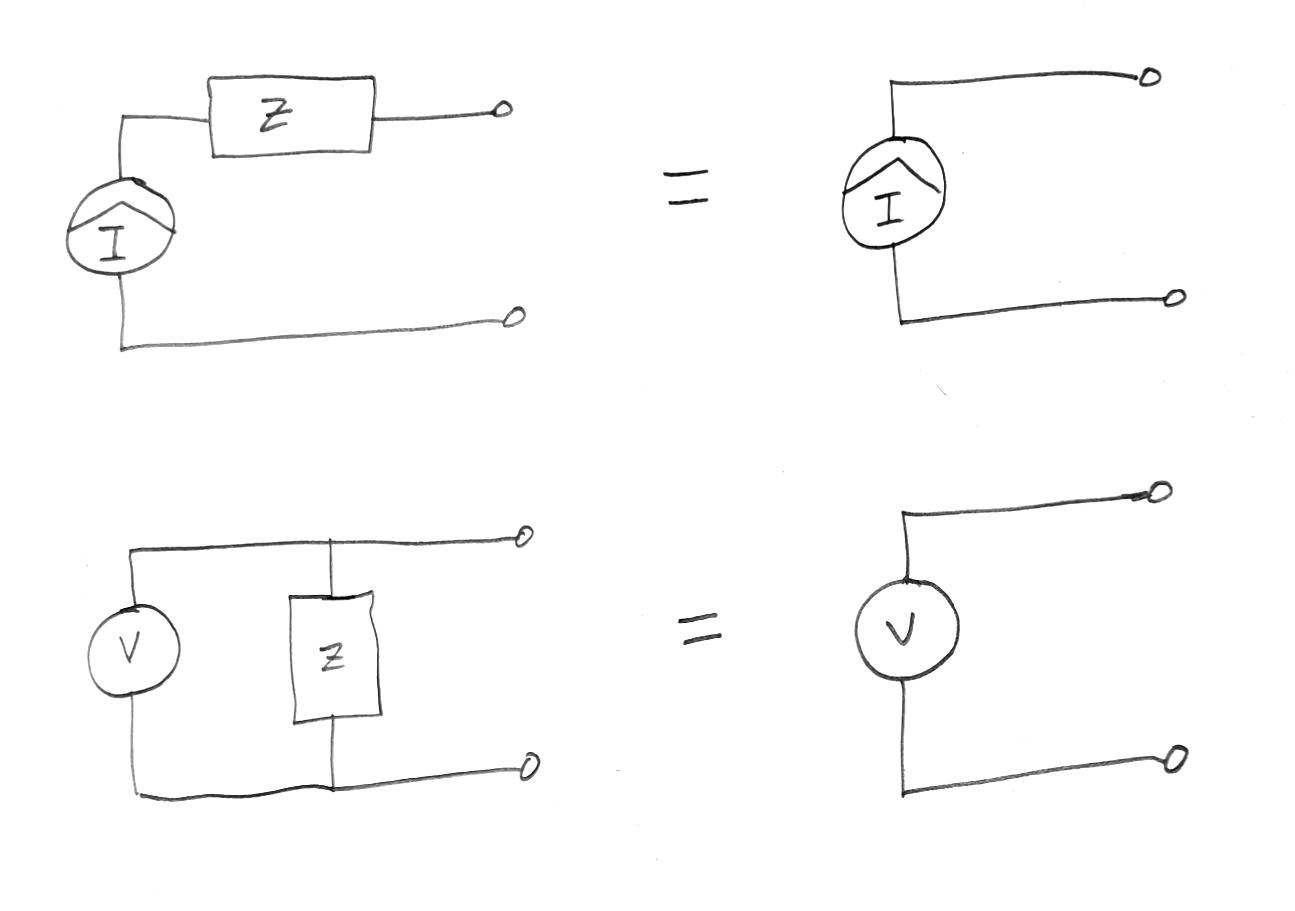
\includegraphics[width=100mm]{figsChapt02/SA35824.png}

Notice that in both cases, the impedance makes no difference in terms of
the output of the circuit for any possible load connection!  That's because the sources
are ``ideal''.   We can apply this to simplify the circuit quite a bit as follows:

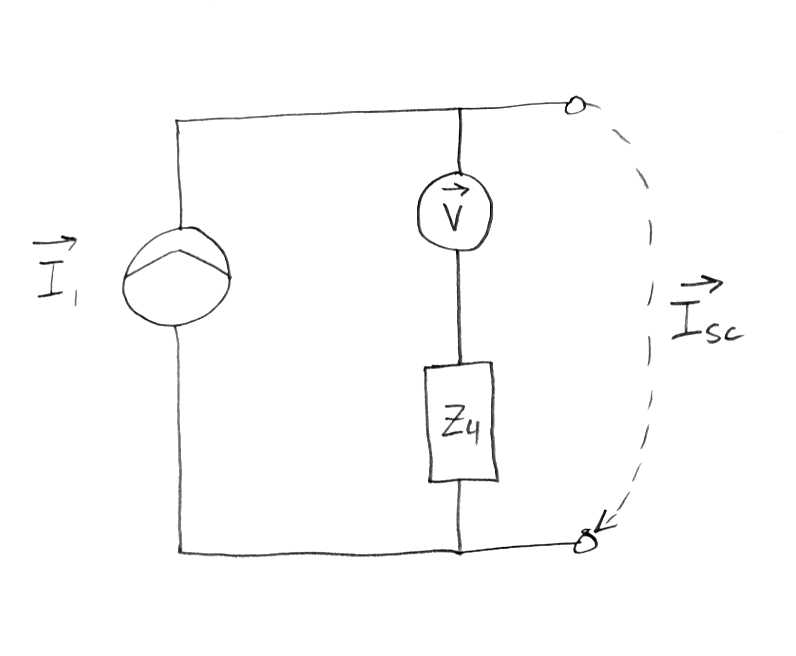
\includegraphics[width=100mm]{figsChapt02/HL67285.png}


First, working on $\vec V_{TH} = \vec V_{OC}$ by going around the loop:
\[ \boxed{
V_{TH} = \vec I_1Z_4+\vec V
}
\]

\end{ExampleCont}
\begin{ExampleCont}

Now, adding a short circuit to the output, we look at $\vec I_{SC}$.   Here we take a superposition approach:

1)  Set $\vec I_1 = 0$ giving
\[
\vec I_{SC1} = \frac {\vec V}{Z_4}
\]

2) Set $\vec V = 0$ giving
\[
\vec I_{SC2} = \vec I_1
\]

3) Finally,
\[
\vec I_{SC} = \vec I_{SC1} + \vec I_{SC2} = \vec I_1 +  \frac {\vec V}{Z_4}
\]

Now we get $Z_{TH}$ by
\[
Z_{TH} = \frac {\vec V_{OC}} {\vec I_{SC}} = \frac  {\vec I_1Z_4+\vec V}  {\vec I_1 +  \frac {\vec V}{Z_4}}
\]
\[
Z_{TH} = Z_4  \frac  {\vec I_1Z_4+\vec V}  {\vec I_1Z_4 +  \vec V}
\]
\[\boxed{Z_{TH} = Z_4  }
\]


Finally we work out the requested answer, $\vec I_5$:

\[
\vec I_5 = \frac {\vec V_{TH}} {Z_{TH} + Z_5}
\]
\[\boxed{
\vec I_5 =  \frac{\vec I_1Z_4 + \vec V}  {Z_4+Z_5}   }
\]

\end{ExampleCont}
%


**************************************************  BH Stopped here (10/8/25)




\section{Simultaneous Equations for Multiple Loops}

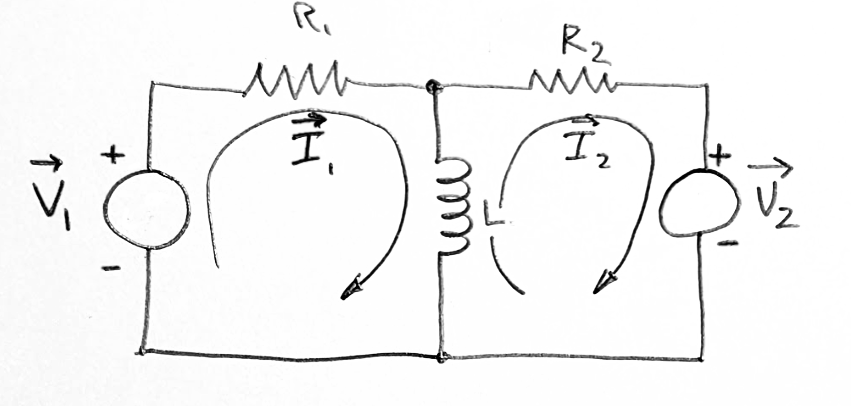
\includegraphics[width=0.33\textwidth]{figsChapt02/KT62219.png}


\subsection*{Problem:}
Find $\vec{I}_1$ and $\vec{I}_2$

\subsection*{Solution:}
Step 1) Write the 2 mesh (loop) equations

\[-\vec{V}_1 + \vec{I}_1 R_1 + j\omega L(\vec{I}_1 - \vec{I}_2) = 0\]

\[\vec V_2 + \vec{I}_2 R_2 + j\omega L(\vec{I}_2 - \vec{I}_1) = 0\]

Step 2) Organize by circuit variables

\[(R_1 + j\omega L)\vec{I}_1 - j\omega L\vec{I}_2 = \vec V_1\]

\[-j\omega L\vec{I}_1 + (R_2 + j\omega L)\vec{I}_2 = -\vec V_2\]

3) Solve these 2 simultaneous equations
   \begin{enumerate}
   \item by substitution (N $\leq$ 3)
   \item by Matrices/Cramer's Rule (N $\leq$ 4)
   \item by Computer (N $>$ 2)($\geq 2$ ?)
   \end{enumerate}

\section*{Note on Matrix Construction}

Factor 2 into:

\[
{Z}{\vec{I}} = \vec{V}\]

e.g.
\[\begin{bmatrix}
R_1 + j\omega L & -j\omega L \\
-j\omega L & R_2 + j\omega L
\end{bmatrix}
\begin{bmatrix}
\vec{I}_1 \\
\vec{I}_2
\end{bmatrix}
=
\begin{bmatrix}
\vec \vec V_1 \\
-\vec \vec V_2
\end{bmatrix}\]

\subsection*{Notes:}
\begin{itemize}
\item $Z_{11}, Z_{22}, Z_{33} \rightarrow$ the diagonal elements, are the sum of all impedances in loop i.
\item For simple impedance like $ Z_{12} $ in other words $Z_{ij}$, the off diagonal
elments are the (negative of the) impedances which couple two loops (i.e. loop 1 to loop 2).
\item  The lower diagonal same as upper  diagonal, e.g. $Z_{13} = Z_{31}$
\end{itemize}

\textbf{The above are ways to check for a correct impedance matrix.}

\paragraph{Solving by Substitution}

From the matrix form above, let $Z_{21}$ be the term at row 2 col 1 of Z

% n.b. $Z_{12} = Z_{21} = -j\omega L$, Row 2, Col 1

\[\vec{I}_1 = \frac{\vec V_1 - Z_{12}\vec{I}_2}{Z_{11}}\]

\[\frac{Z_{21}}{Z_{11}} \vec{V}_1 - \frac{Z_{21}Z_{12}}{Z_{11}}\vec{I}_2 + Z_{22}\vec{I}_2 = -\vec{V}_2\]

\[\vec{I}_2\left(Z_{22} - \frac{Z_{21}Z_{12}}{Z_{11}}\right) = -\frac{Z_{21}}{Z_{11}}\vec V_1 - \vec V_2\]

\[\vec{I}_2 = \frac{-\frac{Z_{21}}{Z_{11}}\vec V_1 - \vec V_2}{Z_{22} - \frac{Z_{21}Z_{12}}{Z_{11}}} = \frac{-Z_{21}\vec V_1 - Z_{11}\vec V_2}{Z_{11}Z_{22} - Z_{21}Z_{12}}\]

\[\vec{I}_1 = \frac{1}{Z_{11}}\vec V_1 - \frac{Z_{12}}{Z_{11}} \frac{-Z_{21}\vec V_1 - Z_{11}\vec V_2}{Z_{11}Z_{22} - Z_{21}Z_{12}}\]

\[= \frac{1}{Z_{11}}\vec V_1 + \frac{Z_{12}Z_{21}\vec V_1 + Z_{12}Z_{11}\vec V_2}{Z_{11}(Z_{11}Z_{22} - Z_{21}Z_{12})} + \frac{Z_{12} \vec V_2}{Z_{11}Z_{22} - Z_{21}Z_{12}}\]

\[= \vec V_1 \frac{(Z_{11}Z_{22} - Z_{21}Z_{12}) + Z_{12}Z_{21}}{Z_{11}(Z_{11}Z_{22} - Z_{21}Z_{12})} + \vec V_2 \frac{Z_{12}}{Z_{11}Z_{22} - Z_{21}Z_{12}}\]

\[\vec{I}_1 = \frac{Z_{22}\vec V_1 + Z_{12}\vec V_2}{Z_{11}Z_{22} - Z_{21}Z_{12}}\]

\subsection{More Complicated Network Example}


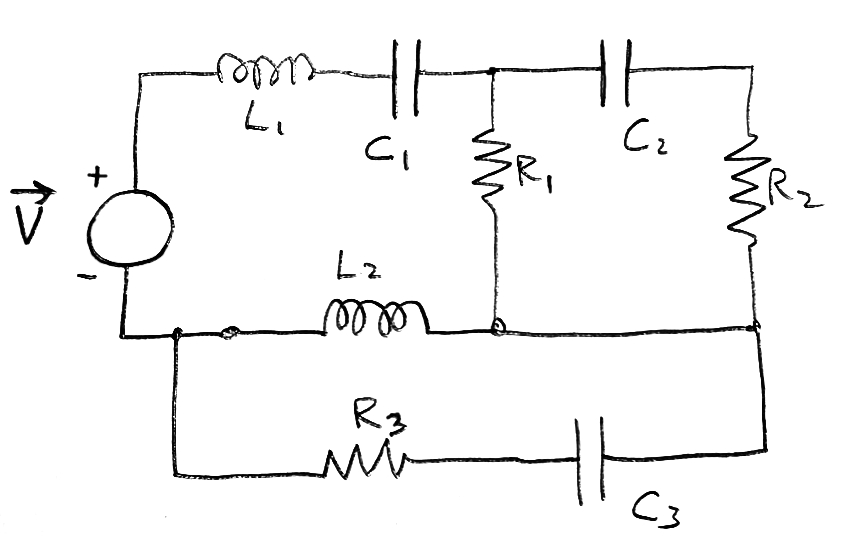
\includegraphics[width=0.6\textwidth]{figsChapt02/EU33724.png} % 10/1/25s

\begin{align*}
L1 &= 2.5 H\\
L2 &= 2.5 H\\
C1 = C2 &= 1/40 F\\
C3 &= 1/80 F\\
R1 = R1 &= 10\Omega\\
R3 &= 5\Omega
\end{align*}

\paragraph{Problem:} Solve the entire circuit to find (for example, $V_0$, $\vec{I}_3$, R)
\vspace{0.2in}

Step 0)  Compute the impedance of each component and re-label the schematic:


\[\omega = 4, L = 2.5H
\]
\[j\omega L =  j10
\]
\[4L = \frac{1}{4C} = 10
\]
\[L = 2.5
\]
\[
C = \frac{1}{40}
\]
\[
\frac{1}{j\omega C} = -j10
\]


Now we place these impedances onto the schematic, and add current loops:

\vspace{0.2in}
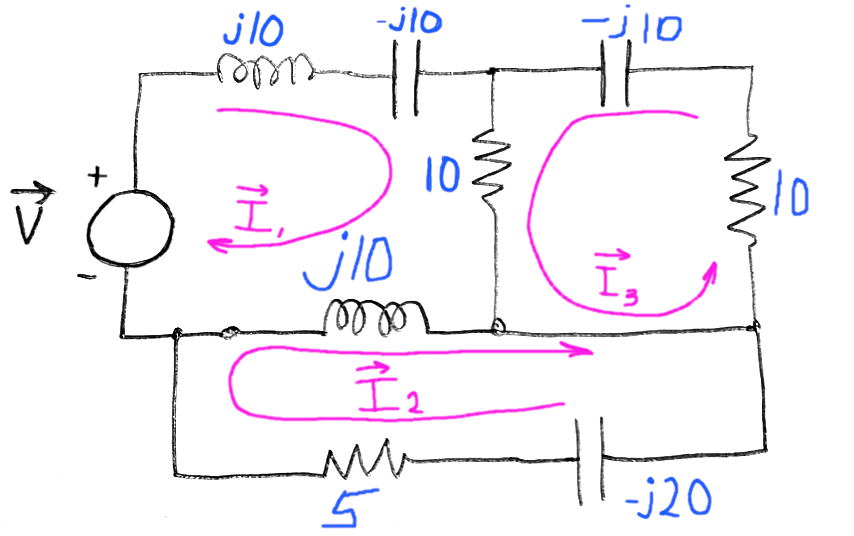
\includegraphics[width=0.6\textwidth]{figsChapt02/LK37610.png} % 10/1/25s

{\bf Note: }   The usual best practice is to make all your current loops either
clockwise or counter clockwise.   However this not a strict requirement.  Because
$\vec I_3 $ is different from the other two, we will just have to watch our signs
a little more carefully below!


\vspace{0.2in}
1) Write 3 Mesh equations
%(N.B.: $j\omega L = j4(2.5),\;\; \frac{1}{j\omega C} = -\frac{j40}{4}$)

  \[
  -V + (j10 - j10)\vec{I}_1 + (\vec I_1 + \vec{I}_3)10 + (\vec{I}_1 - \vec{I}_2)j10 = 0
  \]

  \[
  -j20\vec{I}_2 + 5\vec{I}_2 + j10(\vec{I}_2 - \vec{I}_1) = 0
  \]

  \[
 -j10\vec{I}_3 + 10(\vec{I}_3 + \vec{I}_1) + \vec{I}_3 10 = 0
  \]

2) Arrange:
  \[
  (10 + j10)\vec{I}_1 + (-j10)\vec{I}_2 + (10)\vec{I}_3 = V
  \]
  \[
  (-j10)\vec{I}_1 + (5 - j10)\vec{I}_2 + (0)\vec{I}_3 = 0
  \]
  \[
  (10)\vec{I}_1 + (0)\vec{I}_2 + (20 - j10)\vec{I}_3 = 0
  \]

3) Solve:
\[Z = \begin{bmatrix}
10 + j10 & -j10 & 10 \\
-j10 & 5 - j10 & 0 \\
10 & 0 & 20 - j10
\end{bmatrix}\]

Symmetry check: {\bf PASS}

\vspace{0.2in}
This result gives us the final matrix equation:

\[
Z\vec{I} = \vec{V}
\]

We can, for example, now solve for the currents by
\[
\vec I = (Z^{-1}) \vec V
\]
(using python for example which makes easy work of inverting the 3x3 matrix.)

\paragraph{Alternate method}

Let's get Z even more directly:

Diagonal: $Z_{ii}$ are sums of impedances around each loop:
\[Z_{11} = j10 + (-j10) + 10 + j10 = j10 + j10\]
\[Z_{22} = -j20 + 5 + j10 = 5 - j10\]
\[Z_{23} = 10 - j10 + 10 = 20 - j10\]

Off Diagonal: $Z_{ij}$ = impedance common to both loops $i$ and $j$ (negating the term
if the two current loops go in opposite directions.)
% \& j (- sign (j))wrt $\vec{I}_i$ and $\vec{I}_j$

\[
Z_{12} = j10 -1
\]
$\vec{I}_1, \vec{I}_2$ have opposite signs

\[
Z_{13} = j0 \times +1
\]
$\vec{I}_1, \vec{I}_3$ have same sign

\[
Z_{23} = 0 \times +1 = 0
\]

Same result as above.
Fill in the lower half by symmetry!



